\documentclass[11pt]{article}
\usepackage[margin=1.1in]{geometry}
\usepackage[sc]{mathpazo}
\linespread{1.06}
\usepackage{amsmath,amssymb,amsthm,mathtools}
\usepackage{microtype}
\usepackage{enumitem,booktabs,array}
\usepackage{tikz}
\usetikzlibrary{arrows.meta,positioning,calc,fit}
\usepackage{xcolor}
\usepackage[most]{tcolorbox}
\definecolor{linkblue}{RGB}{25,63,105}
\definecolor{ideabg}{RGB}{244,241,232}
\definecolor{idearule}{RGB}{150,120,60}
\usepackage[colorlinks=true,allcolors=linkblue]{hyperref}
\usepackage[nameinlink,capitalise,noabbrev]{cleveref}
\hypersetup{pdftitle={The Unique Games Theorem: An Expository Account},
  pdfsubject={Expository rewrite of OpenAI's manuscript The Unique Games Theorem (2026)}}

\newtheorem{theorem}{Theorem}[section]
\newtheorem{lemma}[theorem]{Lemma}
\newtheorem{proposition}[theorem]{Proposition}
\newtheorem{corollary}[theorem]{Corollary}
\newtheorem{fact}[theorem]{Fact}
\theoremstyle{definition}
\newtheorem{definition}[theorem]{Definition}
\newtheorem{example}[theorem]{Example}
\theoremstyle{remark}
\newtheorem{remark}[theorem]{Remark}

\newtcolorbox{idea}[1][]{enhanced,breakable,colback=ideabg,colframe=idearule,
  boxrule=0pt,leftrule=2.5pt,arc=0pt,outer arc=0pt,left=8pt,right=8pt,top=5pt,bottom=5pt,
  fonttitle=\bfseries\small,coltitle=idearule!70!black,
  title={#1},attach title to upper={\ \ },before skip=10pt,after skip=10pt}

\newcommand{\F}{\mathbb F}
\newcommand{\E}{\mathbb E}
\newcommand{\eps}{\varepsilon}
\newcommand{\V}{\mathcal V}
\newcommand{\cE}{\mathcal E}
\newcommand{\cG}{\mathcal G}
\newcommand{\cA}{\mathcal A}
\newcommand{\cS}{\mathcal S}
\newcommand{\rs}{r_{\mathrm s}}
\newcommand{\bpi}{\bar\pi}
\DeclareMathOperator{\OPT}{OPT}
\DeclareMathOperator{\val}{val}
\DeclareMathOperator{\Hom}{Hom}
\DeclareMathOperator{\im}{im}
\DeclareMathOperator{\rank}{rank}
\DeclareMathOperator{\Span}{span}
\DeclareMathOperator{\TV}{TV}
\DeclareMathOperator{\Tr}{Tr}
\DeclareMathOperator{\Mat}{Mat}
\newcommand{\abs}[1]{\lvert #1\rvert}
\newcommand{\ip}[2]{\langle #1,#2\rangle}
\setlist{topsep=3pt,itemsep=2pt,parsep=0pt}
\allowdisplaybreaks[1]
\setlength{\emergencystretch}{2em}

\title{\textbf{The Unique Games Theorem}\\[4pt]
\large An expository account of the proof}
\author{A rewrite, for human readers, of the manuscript \emph{The Unique Games Theorem}\\
(OpenAI, September 23, 2026)\\[6pt]
\small Prepared with Claude (Anthropic) \quad$\cdot$\quad October 7, 2026}
\date{}

\begin{document}
\maketitle

\begin{abstract}
\noindent
In September 2026 OpenAI posted a manuscript, written by an internal model, that
proves Khot's Unique Games Conjecture by a deterministic polynomial-time
reduction from 3SAT. The manuscript is complete but compressed: definitions,
estimates and parameter choices arrive in the order the proof needs them, with
little explanation of why they are there. This note presents the same proof for
a reader who knows the PCP theorem, long codes and the outline of the 2-to-2
Games theorem but has not read the manuscript. It explains what each step is
for, does every key calculation in full, gives complete proofs of the one
genuinely new ingredient (a ``latent alphabet gadget''), and sketches the parts
that adapt known machinery, with pointers to the original. It is an exposition,
not a referee report; \cref{sec:reader} lists what was and was not checked and
where a careful reader should concentrate.
\end{abstract}

{\small\setlength{\parskip}{0pt}\tableofcontents}
\clearpage

\section{Introduction}\label{sec:intro}

\subsection{The statement}

A \emph{Unique Games instance} consists of a finite set of vertices, a finite
alphabet $K$, and a list of constraints $e=(u_e,v_e,\pi_e)$, where each
$\pi_e$ is a permutation of $K$. A labeling $\lambda$ satisfies $e$ when
$\lambda(v_e)=\pi_e(\lambda(u_e))$; the value $\val(G)$ is the largest
fraction of constraints a labeling can satisfy. Every label at one end of a
constraint allows exactly one label at the other end, which is what makes a
perfectly satisfiable instance easy: fix one label per connected component and
propagate. The Unique Games Conjecture~\cite{Khot02} says that \emph{nearly}
satisfiable instances are nevertheless hard.

\begin{theorem}[Unique Games Theorem; Theorem~1.1 of \cite{OpenAI-UGC}]\label{thm:ugc}
For all fixed $\eps,\delta\in(0,1/2)$ there are an integer $s\ge1$ and a
deterministic polynomial-time reduction mapping a 3CNF formula $\varphi$ to an
explicit unweighted Unique Games instance $G_\varphi$ over the alphabet
$K=\F_2^s$ such that
\[
\varphi\text{ satisfiable}\ \Rightarrow\ \val(G_\varphi)\ge1-\eps,
\qquad
\varphi\text{ unsatisfiable}\ \Rightarrow\ \val(G_\varphi)\le\delta.
\]
The constraint graph is simple and bipartite, and every constraint is a
translation $\lambda(v_e)=\lambda(u_e)+c_e$ in $\F_2^s$.
\end{theorem}

This is the usual form of the conjecture: both errors are fixed first, and
the alphabet is allowed to depend on them. Through the reductions of
Khot--Kindler--Mossel--O'Donnell~\cite{KKMO07}, Khot--Regev~\cite{KhotRegev},
Raghavendra~\cite{Raghavendra08} and others, the theorem makes the
Goemans--Williamson ratio for Max-Cut, factor~2 for Vertex Cover, and the
basic-SDP threshold for every Max-CSP NP-hard to beat. \Cref{sec:consequences}
lists these.

\subsection{Where things stood, and what was missing}

The 2-to-2 Games theorem of Khot, Minzer and Safra~\cite{KMS17,KMS23}, built on
Dinur--Khot--Kindler--Minzer--Safra~\cite{DKKMS} and
Barak--Kothari--Steurer~\cite{BKS18}, gives NP-hardness of distinguishing
Unique Games of value about $1/2$ from value $\delta$. Two facts frame
the remaining problem.

\begin{enumerate}
\item \textbf{The soundness side is not the problem.} Because the
  parallel-repetition bounds of Rao~\cite{Rao11} and
  Dinur--Steurer~\cite{DS14} for projection games do not depend on the
  alphabet size, it suffices to prove hardness of distinguishing value
  $\ge1-\eps$ from value $\le 1-c$ for one \emph{fixed} $c>0$ and \emph{every}
  $\eps>0$. Repeating $t=t(c,\delta)$ times drives $1-c$ below $\delta$ while
  completeness drops only to $1-t\eps$, and $\eps$ can be chosen after $t$.
  (\Cref{sec:amplify} does this calculation.)
\item \textbf{The completeness side is the problem.} The shortcode test that
  underlies the 2-to-2 theorem has an honest pass probability of only about
  $1/2$ once it is forced to be a permutation test. \Cref{sec:barrier}
  explains why.
\end{enumerate}

So what is needed is a test whose honest strategies pass with probability
$1-p_*$ for arbitrarily small $p_*$, while every labeling that passes with
probability $0.99$ can still be decoded. The manuscript does exactly this.

\subsection{The proof on one page}\label{sec:onepage}

\begin{enumerate}[leftmargin=*]
\item \textbf{Start} from H{\aa}stad's 3LIN gap~\cite{Hastad01}: weighted
  systems of parity equations on three variables, value $\ge1-\xi$ versus
  $\le1/2+\xi$. View it as the usual equation-versus-variable projection
  game, which has value $\le14/15$ in the NO case (\cref{sec:outer}).

\item \textbf{Inner code.} An answer to a tuple $U$ of $k$ equations is a
  vector $z\in\F_2^m$ ($m=1+2k$, homogeneous coordinates). In the
  Barak--Kothari--Steurer (BKS) shortcode, $z$ is encoded by the function
  $M\mapsto Mz$ on $\ell\times m$ binary matrices, and the test compares $M$
  with a rank-one perturbation $M+al^\top$. Honest functions change with
  probability about $1/2$.

\item \textbf{The new idea: a nonlinear decoder.} Replace the target space
  $K=\F_2^\ell$ by a much larger space $\V\supseteq K$ and encode $z$ by
  $P\mapsto C(Pz)$, where $P\colon\F_2^m\to\V$ is linear and
  $C\colon\V\to K$ is a fixed \emph{nonlinear} map that commutes with
  translations by $K$. Perturb $P$ by $al^\top$ with $a$ drawn from a special
  noise law $\mu$ on $\V$. The gadget lemma (\cref{sec:gadget}) builds $C$
  and $\mu$ so that
  \begin{itemize}
  \item $C$ almost never notices the noise: $\Pr[C(x+a)\ne C(x)]\le p_*$;
  \item every family of linear functionals whose restriction to $K$ has rank
    at least a threshold $r_*$ notices the noise with probability $\ge1/8$;
  \item and, crucially, $r_*$ depends only on $p_*$, not on $\ell=\dim K$.
  \end{itemize}
  Honest tables therefore pass with probability $\ge1-p_*/2$.

\item \textbf{Soundness, step 1: back to the ordinary test.} In the Fourier
  expansion over tables, the new noise multiplies each coefficient by a number
  in $[0,1]$ that is at most $7/8$ on ``high-rank'' frequencies. So a labeling
  passing with probability $0.99$ has most of its Fourier mass at rank
  $<r_*$, and therefore passes the \emph{ordinary} BKS equality test with
  probability at least about $2^{-r_*}$, a constant independent of $\ell$
  (\cref{sec:spectral}).

\item \textbf{Soundness, step 2: structure.} The inverse shortcode theorem,
  derived from the Khot--Minzer--Safra Grassmann expansion
  theorem~\cite{KMS23}, says such a function agrees with an affine function
  $Mz+u$ on a slice cut out by a bounded number $\rs$ of row and column
  conditions (\cref{sec:inverse}).

\item \textbf{Soundness, step 3: decoding.} As in the 2-to-2 proof, this
  structure is turned into strategies for a smooth equation-versus-variable
  game in which both players receive a little shared linear ``advice''. The
  strategies agree with probability $\gamma>0$, independent of the tuple
  length $k$ (\cref{sec:decoding}).

\item \textbf{Soundness, step 4: contradiction.} On many coordinates
  (``clean'' ones) the advice says nothing, and there the players are
  playing the original game in parallel. Parallel repetition bounds their
  agreement by $\exp(-ck^{1/3})$, which is below $\gamma$ for large $k$
  (\cref{sec:clean}).

\item \textbf{Finish.} The resulting game has completeness $1-k\xi-p_*/2$ and
  soundness $0.99$. Remove weights, make it simple and bipartite, and apply
  $t$-fold parallel repetition (\cref{sec:finish}).
\end{enumerate}

\begin{figure}[t]
\centering
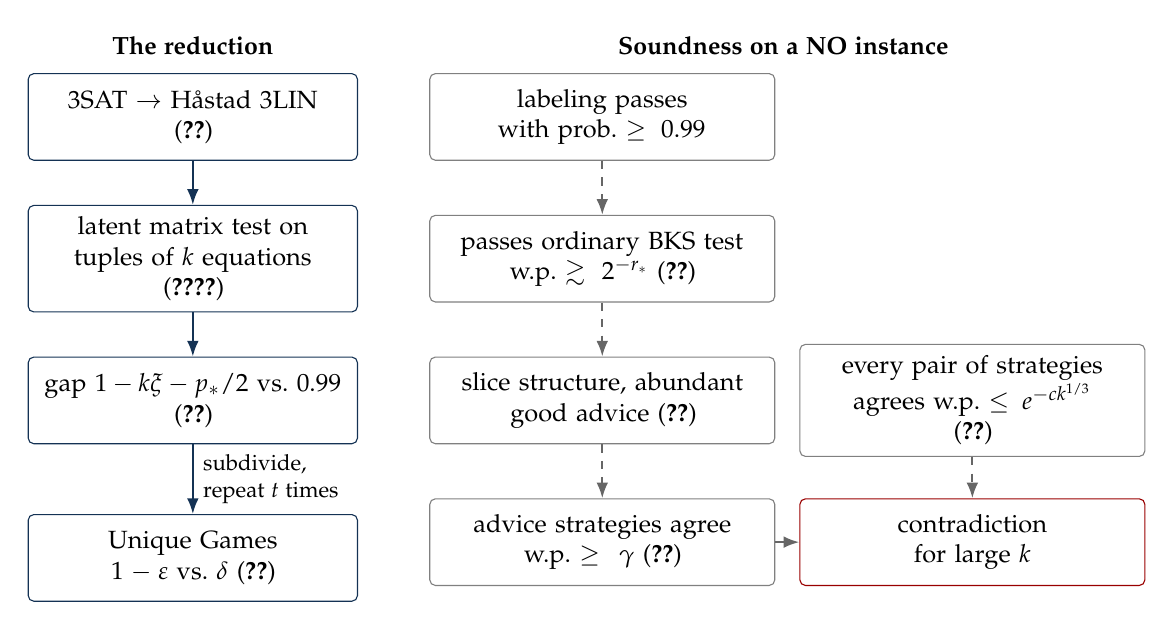
\begin{tikzpicture}[x=1cm,y=1cm,every node/.style={font=\small},
  box/.style={draw=linkblue!80!black,rounded corners=2pt,align=center,inner sep=4pt,text width=3.9cm,minimum height=11mm},
  sbox/.style={draw=black!50,rounded corners=2pt,align=center,inner sep=4pt,text width=4.1cm,minimum height=11mm},
  arr/.style={-{Latex[length=2mm]},thick,draw=linkblue!80!black},
  dsh/.style={-{Latex[length=2mm]},thick,dashed,draw=black!60}]
\node[font=\small\bfseries] at (0,0.9) {The reduction};
\node[font=\small\bfseries] at (7.5,0.9) {Soundness on a NO instance};
\node[box] (a) at (0,0) {3SAT $\to$ H{\aa}stad 3LIN\\ (\cref{sec:outer})};
\node[box] (b) at (0,-1.8) {latent matrix test on\\ tuples of $k$ equations\\ (\cref{sec:gadget,sec:instance})};
\node[box] (c) at (0,-3.6) {gap $1-k\xi-p_*/2$ vs.\ $0.99$\\ (\cref{prop:gap})};
\node[box] (d) at (0,-5.6) {Unique Games\\ $1-\eps$ vs.\ $\delta$ (\cref{sec:finish})};
\draw[arr] (a)--(b); \draw[arr] (b)--(c);
\draw[arr] (c)-- node[right,font=\footnotesize,align=left]{subdivide,\\ repeat $t$ times} (d);
\node[sbox] (s1) at (5.2,0) {labeling passes\\ with prob.\ $\ge0.99$};
\node[sbox] (s2) at (5.2,-1.8) {passes ordinary BKS test\\ w.p.\ $\gtrsim2^{-r_*}$ (\cref{sec:spectral})};
\node[sbox] (s3) at (5.2,-3.6) {slice structure, abundant\\ good advice (\cref{sec:inverse})};
\node[sbox] (s4) at (5.2,-5.4) {advice strategies agree\\ w.p.\ $\ge\gamma$ (\cref{sec:decoding})};
\node[sbox] (s5) at (9.9,-3.6) {every pair of strategies\\ agrees w.p.\ $\le e^{-ck^{1/3}}$\\ (\cref{sec:clean})};
\node[sbox,draw=red!60!black] (s6) at (9.9,-5.4) {contradiction\\ for large $k$};
\draw[dsh] (s1)--(s2); \draw[dsh] (s2)--(s3); \draw[dsh] (s3)--(s4);
\draw[dsh] (s4)--(s6); \draw[dsh] (s5)--(s6);
\end{tikzpicture}
\caption{Roadmap. Solid arrows: the reduction. Dashed arrows: the soundness
argument, which plays a decoding lower bound against a repetition upper bound.}
\label{fig:roadmap}
\end{figure}

\subsection{What is new and what is inherited}

Most of the soundness argument adapts known machinery: H{\aa}stad's 3LIN
hardness, the BKS matrix formulation of the shortcode, the KMS Grassmann
expansion theorem, the smooth outer game with shared linear advice of
Khot--Minzer--Safra and Minzer--Zheng~\cite{KMS17,MZ}, Khot--Safra's
``virtual tables'' and Fourier list decoding~\cite{KS13}, folding in the style of
Bellare--Goldreich--Sudan~\cite{BGS98}, and Dinur--Steurer
repetition~\cite{DS14}. The new ingredients are:

\begin{itemize}
\item \textbf{The latent alphabet gadget} (\cref{sec:gadget}), a nonlinear,
  translation-equivariant map that is stable under a noise that every
  high-rank linear observer detects. This is what breaks the completeness
  barrier. Its proof is elementary (finite fields, a polynomial-identity
  argument, and a potential function) and is given here in full.
\item \textbf{Exact table keys} (\cref{sec:keys}): tables on a tuple and on its
  sparse projection are identified exactly, so the projected player's answers
  come from the same labeling and no separate consistency test is needed.
\item \textbf{An erasure argument} (\cref{sec:abundance}) showing that the
  structure promised by the inverse theorem is visible from \emph{random}
  advice with constant probability, not merely that it exists somewhere.
\item The realization, visible in the model's released reasoning summary, that
  a \emph{fixed} soundness gap with completeness tending to $1$ suffices,
  which makes a constant-factor damping of high-rank Fourier mass enough.
\end{itemize}

\subsection{Formal verification}\label{sec:lean}

The repository includes a Lean~4 formalization of this result (directory
\nolinkurl{lean/OAI/Computability/UniqueGames}, about 480 files and 187{,}000
lines) and a Comparator challenge file \texttt{UniqueGamesTheorem.lean} that
states the theorem using only Mathlib. That statement asserts, for real
$0<\eps,\delta<1/2$, the existence of a reduction from the binary-encoded
language of satisfiable 3CNF formulas, computable in polynomial time by a
Mathlib \texttt{TM2} Turing machine, to simple bipartite translation
instances over $\F_2^s$ with completeness $1-\eps$ and soundness $\delta$.
The permitted axioms are the three standard ones (\texttt{propext},
\texttt{Quot.sound}, \texttt{Classical.choice}). The file names indicate that
the external inputs (H{\aa}stad's verifier, the KMS expansion theorem,
projection-game repetition) are formalized rather than assumed. I read the
challenge statement but did not run the check, which requires building the
whole development.

\subsection{How this note is organized}

\Cref{sec:reductions} reduces the theorem to a fixed-gap statement.
\Cref{sec:gadget} builds the gadget. \Cref{sec:instance} defines the Unique
Games instance and proves completeness. \Cref{sec:plan} states the two bounds
that make up soundness, and
\cref{sec:spectral,sec:inverse,sec:decoding,sec:clean} prove them.
\Cref{sec:finish} assembles the parameters. \Cref{sec:reader} is a guide for
checking the proof, with a table matching this note to the manuscript.
Throughout, vector spaces are over $\F_2$ unless stated otherwise, $E^*$
denotes the dual of $E$, and ``uniform'' sampling from a vector space
includes $0$.

\section{Two easy reductions}\label{sec:reductions}

\subsection{A fixed gap is enough}\label{sec:amplify}

The whole proof aims at a weighted translation game with completeness
arbitrarily close to $1$ and soundness at most $0.99$. This subsection shows
why that suffices. Two standard tools are used.

\begin{theorem}[Projection-game repetition; Dinur--Steurer~{\cite[Cor.~1.2]{DS14}}]\label{thm:repetition}
Let $G$ be a finite bipartite projection game with any probability
distribution on its constraints. If $\val(G)\le1-g$, then for every $n\ge1$,
$\val(G^{\otimes n})\le(1-g^2/16)^n$. The bound does not depend on the
alphabet or on the number of questions.
\end{theorem}

A unique game is a projection game, and the $n$-fold product of translation
constraints with offsets $c_1,\dots,c_n$ is the translation by
$(c_1,\dots,c_n)$ on $K^n$, so repetition stays inside the class of
translation games.

\begin{lemma}[Rounding and subdivision; Lemma~7.1 of \cite{OpenAI-UGC}]\label{lem:subdivide}
Let $H$ be a permutation game with $h$ constraint occurrences carrying positive
rational weights summing to $1$ (loops and parallel occurrences allowed). For
rational $\tau>0$ one can build in polynomial time an unweighted simple
bipartite game $B$ on the same alphabet, with $4\lceil h/\tau\rceil$ edges, such
that
\[
\Bigl|\val(B)-\Bigl(1-\tfrac{1-\val(H)}{4}\Bigr)\Bigr|\le\tfrac\tau4 .
\]
Translation constraints stay translation constraints.
\end{lemma}

\begin{proof}[Proof idea]
Round the weights to multiples of $1/Q$ with $Q=\lceil h/\tau\rceil$ by
largest remainders and replace each occurrence by that many copies; this
changes the value by at most $h/(2Q)\le\tau$. Then replace each occurrence
$u\to v$ with constraint $\rho$ by a path $u-p-q-r-v$ through three fresh
vertices, with identity constraints on the first three edges and $\rho$ on the
last. A satisfied occurrence extends to four satisfied edges and a violated one
to exactly three, giving $\val(B)=1-(1-\val(H'))/4$ exactly. Putting the
original vertices and the $q$'s on one side and the $p$'s and $r$'s on the
other makes $B$ bipartite, and fresh interiors make it simple.
\end{proof}

\begin{corollary}\label{cor:amplify}
Suppose that for every rational $d>0$ there is a polynomial-time reduction from
3SAT to weighted translation games $H$ over some alphabet $\F_2^{\ell}$
(allowed to depend on $d$) with
\[
\text{YES: }\val(H)\ge1-d,\qquad \text{NO: }\val(H)\le 99/100 .
\]
Then \cref{thm:ugc} holds.
\end{corollary}

\begin{proof}
Fix $\eps,\delta$. Apply \cref{lem:subdivide} with $\tau\le1/200$; in the NO
case $\val(B)\le1-(1/100-\tau)/4\le1-1/800$. With $g=1/800$,
\cref{thm:repetition} gives $\val(B^{\otimes t})\le(1-1/10{,}240{,}000)^t$,
so choose $t$ (depending only on $\delta$) to make this at most $\delta$.
\emph{Only now} choose $d\le\eps/t$ and $\tau\le\min\{1/200,\eps/t\}$. In the
YES case $\val(B)\ge1-(d+\tau)/4$, and labeling $B^{\otimes t}$
coordinatewise gives, by a union bound,
$\val(B^{\otimes t})\ge1-t(d+\tau)/4\ge1-\eps/2$. The product of simple
bipartite graphs is simple bipartite, and the alphabet is $\F_2^{\ell t}$.
\end{proof}

The order of quantifiers is the whole point: $t$ is fixed by $\delta$ alone,
because the NO gap $1/800$ does not depend on anything, and only then is the
completeness error chosen. Alphabet-independent repetition is essential here,
since the alphabet $\F_2^\ell$ is chosen after $t$.

\subsection{The outer game}\label{sec:outer}

\begin{theorem}[H{\aa}stad~{\cite[Thm.~5.4]{Hastad01}}]\label{thm:parity}
For every rational $\xi>0$ there is a polynomial-time reduction from SAT to
weighted systems $\cE$ of equations $x_{v_1}+x_{v_2}+x_{v_3}=b$ over $\F_2$ such
that $\OPT(\cE)\ge1-\xi$ in the YES case and $\OPT(\cE)\le\frac12+\xi$ in the
NO case.
\end{theorem}

Later arguments need the three variables of each equation to be distinct.

\begin{lemma}[Distinct positions; Lemma~4.2 of \cite{OpenAI-UGC}]\label{lem:distinct}
One can transform $\cE$ in polynomial time into $\cE'$ with three distinct
variables per equation, such that $\OPT(\cE')\ge\OPT(\cE)$ and
$\OPT(\cE')\le\frac{1+\OPT(\cE)}2+\frac3{100}$. In particular, with
$\xi<1/100$ the NO case gives $\OPT(\cE')\le4/5$.
\end{lemma}

\begin{proof}[Proof idea]
Replace each variable by $100$ clones and each equation by all ways of choosing
clones for its positions (distinct clones where the same variable repeats),
with equal conditional weights. Completeness is clear. For soundness, let
$t_v\in[-1,1]$ be the average of $(-1)^{x}$ over the clones of $v$. With clones
chosen independently, an equation is satisfied with probability
$\tfrac12(1+(-1)^b t_{v_1}t_{v_2}t_{v_3})$. Rounding each $t_v$ to its sign
gives an assignment, and every equation it violates has probability at most
$1/2$, so the average is at most $(1+\OPT)/2$. Conditioning on distinctness
costs at most $3/100$.
\end{proof}

From now on every equation has three distinct variables. The
\emph{equation-versus-variable game} $G_\cE$ picks an equation $e$ by weight and
a position $j\in\{1,2,3\}$ uniformly. One player gets $e$ and answers with one
of the four satisfying assignments of $e$; the other gets the $j$-th variable of
$e$ and answers with a bit; they win if the bits agree. The variable player's
answers form a global assignment, which violates a $1-\OPT$ fraction of
equations, and on each violated equation the equation player disagrees in at
least one of three positions. Hence
\begin{equation}\label{eq:base-gap}
\OPT(\cE)\le\tfrac45\quad\Longrightarrow\quad \val(G_\cE)\le1-\tfrac{1-\OPT}{3}\le\tfrac{14}{15}.
\end{equation}

\section{Breaking the completeness barrier: the latent gadget}\label{sec:gadget}

\subsection{Why the shortcode test has completeness one half}\label{sec:barrier}

In the BKS formulation of the degree-two shortcode, an answer $z\in\F_2^m$ is
encoded by the function $f_z(M)=Mz$ on $\Mat_{\ell,m}=\Hom(\F_2^m,\F_2^\ell)$.
The test picks a uniform matrix $M$ and uniform $a\in\F_2^\ell$,
$l\in\F_2^m$, and compares $M$ with $M+al^\top$. Since
\[
f_z(M+al^\top)=f_z(M)+a\,(l^\top z),
\]
the two values differ exactly when $l^\top z=1$ and $a\ne0$, that is, with
probability about $1/2$. BKS accept if $f(M+al^\top)\in\{f(M),\,f(M)+a\}$,
which honest functions always pass; that is a 2-to-2 test. To get a
\emph{unique} test one must demand equality, and then honest functions pass
only half the time. This is the source of the ``$1/2$'' in the Unique Games
corollary of the 2-to-2 theorem.

The trouble is that the noise $a(l^\top z)$ reaches the codeword at full
strength. The manuscript's idea is to make the codeword blind to most of the
noise while the soundness analysis still sees all of it.

\subsection{A nonlinear decoder}

Replace $\F_2^\ell$ by a larger space $\V$ containing $K=\F_2^\ell$, let
tables be linear maps $P\colon\F_2^m\to\V$, and encode $z$ by
\[
F(P)=C(Pz),
\]
where $C\colon\V\to K$ is a fixed map. For folding we need
$C(x+h)=C(x)+h$ for $h\in K$. Perturb $P$ by $al^\top$ with $a\sim\mu$ for a
noise law $\mu$ on $\V$. Then $Pz$ is a uniform element of $\V$ independent of
$a$ and of the fair bit $l^\top z$, so the honest encoding changes with
probability $\tfrac12\Pr[C(x+a)\ne C(x)]$.

What does soundness need from $\mu$? In the Fourier expansion over tables
(\cref{sec:spectral}), a frequency is a tuple $g=(g_0,\dots,g_{m-1})$ of
functionals $g_i\in\V^*$, and averaging over $l$ shows that the noise
multiplies its coefficient by
\[
\Lambda_g=\Pr_{a\sim\mu}[\,g_i(a)=0\text{ for all }i\,].
\]
For the reduction to the ordinary BKS test we want $\Lambda_g$ bounded away
from $1$ whenever the functionals $g_i$, restricted to $K$, span a space of
large dimension. That is the gadget's second property.

\begin{idea}[Why $C$ must be nonlinear.]
If $C$ were linear with $C|_K=\mathrm{id}$, take $G$ to be the span of the
$\ell$ coordinate functionals of $C$. Its restriction to $K$ has full rank
$\ell$, and some $g\in G$ has $g(a)\ne0$ exactly when $C(a)\ne0$, that is,
exactly when $C(x+a)\ne C(x)$. Stability and detection would be the same
event. So any useful $C$ is nonlinear, and the content of the lemma is that a
nonlinear map can be much more stable than every linear observer of comparable
rank.
\end{idea}

\begin{theorem}[Latent alphabet gadget; Lemma~3.1 of \cite{OpenAI-UGC}]\label{thm:gadget}
For every $p_*>0$ there is an integer $r_*$ such that for every sufficiently
large $\ell$ there are a binary space $\V\supseteq K=\F_2^\ell$, a map
$C\colon\V\to K$ and a probability law $\mu$ on $\V$ with:
\begin{enumerate}[label=(\roman*)]
\item \emph{equivariance:} $C(x+h)=C(x)+h$ for all $x\in\V$, $h\in K$;
\item \emph{stability:} $\Pr[C(x+a)\ne C(x)]\le p_*$ for independent uniform
  $x\in\V$ and $a\sim\mu$;
\item \emph{detection:} every subspace $G\le\V^*$ with $\dim(G|_K)\ge r_*$
  satisfies $\Pr_{a\sim\mu}[\exists g\in G:\ g(a)\ne0]\ge1/8$.
\end{enumerate}
The threshold $r_*$ is fixed before $\ell$, and everything is computable when
$p_*$ is rational.
\end{theorem}

The construction has three layers: a quadratic \emph{block} over a finite field
(\cref{sec:block}); a deep \emph{tree} of blocks with a fixed output space
$B=\F_{2^d}^3$ (\cref{sec:tree,sec:lifts}); and an \emph{enlargement} from
$B$ to an arbitrary $K$ (\cref{sec:enlarge}).

\begin{idea}[The idea in one paragraph: one life versus many lives.]
Think of a noise symbol injected at a random leaf of a deep tree and
propagating upward. At each level the nonlinear output ``absorbs'' the
perturbation with a small probability $\theta$, so after $s$ levels it survives
with probability about $e^{-\theta s}$: one life, lost at rate $\theta$.
A rank-$r$ family of linear observers behaves differently. At each level it can
lose at most \emph{one} dimension, and only with probability at most
$3r\theta$. Measuring rank by the harmonic number $H_r=1+\frac12+\dots+\frac1r$,
the expected loss per level is at most about $3\theta$, so killing all $r$
dimensions takes about $H_r/(3\theta)\approx(\ln r)/(3\theta)$ levels. Taking
$s\approx H_{r_0}/(8\theta)$ levels, the nonlinear output survives with
probability about $r_0^{-1/8}$, which is small when $r_0$ is large, while a
family starting at rank $r_0$ survives with probability at least $1/2$. The
factor $\ln r_0$ is the whole separation.
\end{idea}

\subsection{The quadratic block}\label{sec:block}

Fix $d\ge1$, put $q=2^d$ and $F=\F_q$, and let $X=B=F^3$, regarded as binary
spaces of dimension $b=3d$. Identify $X^*$ and $B^*$ with $F^3$ through the
trace pairing $z\mapsto(y\mapsto\Tr(z\cdot y))$, where $z\cdot y$ is the
$F$-bilinear dot product and $\Tr=\Tr_{F/\F_2}$. Recall that the trace
pairing is nondegenerate, that $\Tr(t^2)=\Tr(t)$, and that every element of $F$
has a unique square root. Define
\[
Q(x_1,x_2,x_3)=(x_2x_3,\;x_1x_3,\;x_1x_2),\qquad
D(x,a)=Q(x+a)+Q(x)+Q(a),
\]
and the block map
\[
C_{\mathrm{blk}}\colon X\oplus B\to B,\qquad C_{\mathrm{blk}}(x,y)=y+Q(x).
\]
It is equivariant in the second (``vertical'') argument:
$C_{\mathrm{blk}}(x,y+h)=C_{\mathrm{blk}}(x,y)+h$.

\paragraph{Update spaces.} For each $F$-line $A=Fv\subseteq F^3$ let
\[
D_A=\{y\in B:\ v\cdot y=0\},\qquad
U_A=\{(a,\;Q(a)+w):\ a\in A,\ w\in D_A\}\subseteq X\oplus B .
\]
There are $q^2+q+1$ lines; set $\theta=1/(q^2+q+1)$.

\begin{lemma}\label{lem:block-basic}
Each $U_A$ is a binary subspace of dimension $b$. For $a\in A$ and any $x$,
$D(x,a)\in D_A$, and $D(a,a')=0$ for $a,a'\in A$. Under the trace pairing the
annihilator of $D_A$ is $A$. The spaces $U_A$ together span $X\oplus B$.
\end{lemma}

\begin{proof}
The coordinates of $D(x,a)$ are $x_2a_3+a_2x_3$, $x_1a_3+a_1x_3$,
$x_1a_2+a_1x_2$. For $a=tv$ every term of $v\cdot D(x,a)$ appears twice, so
it vanishes; and for $a,a'\in A$ each coordinate of $D(a,a')$ vanishes. So $Q$
is additive on $A$, and $(a,w)\mapsto(a,Q(a)+w)$ is a linear bijection
$A\oplus D_A\to U_A$, of dimension $d+2d=b$. Elements of $A$ annihilate $D_A$,
and the annihilator has dimension $3d-2d=d$, so it equals $A$. For the
coordinate lines $Fe_i$, $Q$ vanishes on $Fe_i$, so $U_{Fe_i}$ contains
$Fe_i\oplus0$ and $0\oplus D_{Fe_i}$; these span $X\oplus B$.
\end{proof}

\begin{lemma}[One update; Lemma~3.3 of \cite{OpenAI-UGC}]\label{lem:block-noise}
For uniform $(x,y)$ and an independent uniform nonzero $\zeta\in U_A$,
$\Pr[C_{\mathrm{blk}}((x,y)+\zeta)\ne C_{\mathrm{blk}}(x,y)]=1-\theta$.
\end{lemma}

\begin{proof}
For $\zeta=(a,Q(a)+w)$ the output changes by $Q(a)+w+Q(x+a)+Q(x)=w+D(x,a)$,
which lies in $D_A$. If $\zeta$ is uniform in all of $U_A$, then $w$ is uniform
in $D_A$ and independent of $a$, so the change is uniform in $D_A$ and is zero
with probability $q^{-2}$. The zero update has probability $q^{-3}$, so
conditioning on $\zeta\ne0$ gives change probability
$(1-q^{-2})/(1-q^{-3})=q(q+1)/(q^2+q+1)=1-\theta$.
\end{proof}

So each block absorbs a random update with the small probability $\theta$.
That is the ``one life'' rate.

\paragraph{Linear observers of one block.} A functional on $X\oplus B$
whose restriction to the vertical $B$ is $z\in B^*$ has the form $(\gamma_z,z)$
with $\gamma_z\in X^*$. Fix a subspace $S\le B^*$ and a linear choice
$\gamma\colon S\to X^*$ of extensions; write $\gamma_z(x)=\Tr(g(z)\cdot x)$
with $g\colon S\to F^3$ binary linear. Restricting to an update space gives
\[
\kappa_{A,\gamma}\colon S\to U_A^*,\qquad z\mapsto(\gamma_z,z)|_{U_A}.
\]
An observer ``loses a dimension'' at $A$ when $\kappa_{A,\gamma}$ has a
kernel.

\begin{lemma}[When an observer dies; Lemma~3.4 of \cite{OpenAI-UGC}]\label{lem:kernel}
For nonzero $z\in S$: $\kappa_{A,\gamma}(z)=0$ if and only if $A=Fz$ and
\begin{equation}\label{eq:align}
z\cdot g(z)=\sqrt{z_1z_2z_3}.
\end{equation}
\end{lemma}

\begin{proof}
Vanishing on the vertical vectors $(0,w)$, $w\in D_A$, forces $z\in A$ by
\cref{lem:block-basic}, so $A=Fz$. On the remaining vectors $(tz,Q(tz))$ the
functional equals $\Tr\bigl(t\,g(z)\cdot z+z\cdot Q(tz)\bigr)$, and
$z\cdot Q(tz)=3t^2z_1z_2z_3=t^2z_1z_2z_3$. Since
$\Tr(t^2c)=\Tr(t\sqrt c)$, this is $\Tr\bigl(t(g(z)\cdot z+\sqrt{z_1z_2z_3})\bigr)$,
which vanishes for all $t$ exactly when \eqref{eq:align} holds.
\end{proof}

So two things must go wrong for an observer to lose a dimension: the random line
must be the line through one of its characters, and that character must
satisfy the ``alignment'' equation \eqref{eq:align}. The left side of
\eqref{eq:align} is quadratic in the binary coordinates of $z$, while the right
side is genuinely cubic, so typical subspaces have few aligned characters.

\subsection{Generic subspaces}

\begin{definition}
A binary subspace $S\le F^3$ of dimension $r\ge1$ is \emph{generic} if no two
distinct nonzero elements of $S$ are $F$-proportional, and for every binary
linear $g\colon S\to F^3$ at most $3r$ nonzero $z\in S$ satisfy
\eqref{eq:align}.
\end{definition}

For a generic $S$ and a \emph{fixed} $\gamma$, a uniformly random line $A$
causes a loss only if $A=Fz$ for an aligned $z$, and at most one dimension is
lost (two kernel elements would lie on the same line). Hence, writing $r_A$
for the rank after restriction,
\begin{equation}\label{eq:rank-loss}
r-r_A\le1,\qquad \Pr_A[r_A<r]\le3r\theta,\qquad \E_A[H_r-H_{r_A}]\le3\theta .
\end{equation}
For an arbitrary rank-$r$ space a loss still needs $A=Fz$ for some nonzero
$z\in S$, so $\Pr_A[r_A<r]\le2^r\theta$.

\begin{lemma}[Lemma~3.6 of \cite{OpenAI-UGC}]\label{lem:generic}
For fixed $r$, a uniformly random $r$-dimensional binary subspace of $F^3$ is
generic with probability tending to $1$ as $d\to\infty$.
\end{lemma}

\begin{proof}[Proof sketch]
Parametrize $S$ by independent uniform $x_{ij}\in F$ through
$z_i(t)=\sum_jx_{ij}t_j$ for $t\in\F_2^r$. Non-injectivity and proportional
pairs have probability $O_r(q^{-2})$.

For alignment, fix a set $E$ of $3r+1$ nonzero points $t$. Since $g$ is
determined by its values $g_{ij}$ on a basis, alignment on all of $E$ says
that the vector $c=(\sqrt{z_1(t)z_2(t)z_3(t)})_{t\in E}$ lies in the $F$-span
of the $3r$ columns $M_{t,(i,j)}=t_jz_i(t)$. Treat the $x_{ij}$ as
indeterminates over $L=\F_2(x_{ij})$. Because the square root is additive in
characteristic~$2$ and $t_j\in\{0,1\}$,
\[
c_t=\sum_{j,k,l}t_jt_kt_l\sqrt{x_{1j}x_{2k}x_{3l}},
\]
and the $r^3$ elements $\sqrt{x_{1j}x_{2k}x_{3l}}$ are linearly independent
over $L$ (distinct parity patterns of exponents). If $c$ were in the column span
over $\overline L$, every $L$-row vector killing the columns would kill each
evaluation vector $(t_jt_kt_l)_{t\in E}$, so all of these, which include all
monomials of degree $1,2,3$ (as $t_i^2=t_i$), would lie in the $L$-column span.
But the columns are evaluations of polynomials of degree $\le2$. Then
``degree $\le3$'' $\subseteq$ column span $\subseteq$ ``degree $\le2$'', so
these spaces coincide and are closed under multiplication by each $t_i$, hence
contain all positive-degree monomials, which span $L^E$ because $0\notin E$.
That forces the column span to have dimension $|E|>3r$, a contradiction.

To specialize to $F$, square everything (Frobenius preserves rank): the
augmented matrix then has a nonzero minor of size $\rank+1$ that is a
polynomial of degree $\le6r+3$, while all minors of that size of the
unaugmented matrix vanish identically. By the Schwartz--Zippel bound, column
membership after specialization has probability $\le(6r+3)/q$. A union bound
over the finitely many $E$ finishes the proof.
\end{proof}

Fix $r_0$ (to be chosen from $p_*$), then $\eps_0\in(0,1)$ with
$H_{r_0}2^{r_0}\eps_0\le1$, and then $d$ so large that $3d\ge r_0$ and, for
every $1\le r\le r_0$, a uniform rank-$r$ subspace of $B^*$ is non-generic with
probability at most $\eps_0$. Fix one generic subspace $S_\star$ of rank $r_0$.

\subsection{The tree of blocks}\label{sec:tree}

We now stack blocks, keeping the output space $B$ fixed. We build input spaces
$P_t$, ``shift'' subspaces $R_t\le P_t$ with surjections
$\lambda_t\colon R_t\to B$, and maps $C_t\colon P_t\to B$ satisfying
\begin{equation}\label{eq:tree-equiv}
C_t(u+h)=C_t(u)+\lambda_t(h)\qquad(h\in R_t).
\end{equation}
Start with $P_0=R_0=B$ and $C_0=\lambda_0=\mathrm{id}$. Let $\mathcal I$ be the
set of pairs $(A,J)$, with $A$ a line and $J\colon B\to U_A$ a binary linear
isomorphism. Put $P_t=\prod_{(A,J)\in\mathcal I}P_{t-1}$: one child for
\emph{every} line and every way of identifying the child's output with that
line's update space. Then aggregate and apply one block:
\[
(x,y)=\sum_{(A,J)}J\,C_{t-1}(u_{AJ})\in X\oplus B,\qquad C_t(u)=y+Q(x).
\]
A tuple of child shifts is a parent shift when the $X$-part of its aggregate
vanishes, and then $\lambda_t$ records the $B$-part. Because the $U_A$ span
$X\oplus B$, $\lambda_t$ is onto, and $C_t$ maps uniform inputs to uniform
outputs.

\paragraph{The noise.} $\xi_0$ is a uniform element of $B$. For $t\ge1$, $\xi_t$
picks a uniform child $(A,J)$ and puts an independent copy of $\xi_{t-1}$
there, with zero elsewhere. Equivalently: choose a uniform root-to-leaf path,
one uniform $(A,J)$ per level, and add a uniform symbol of $B$ at that leaf.

\begin{figure}[t]
\centering
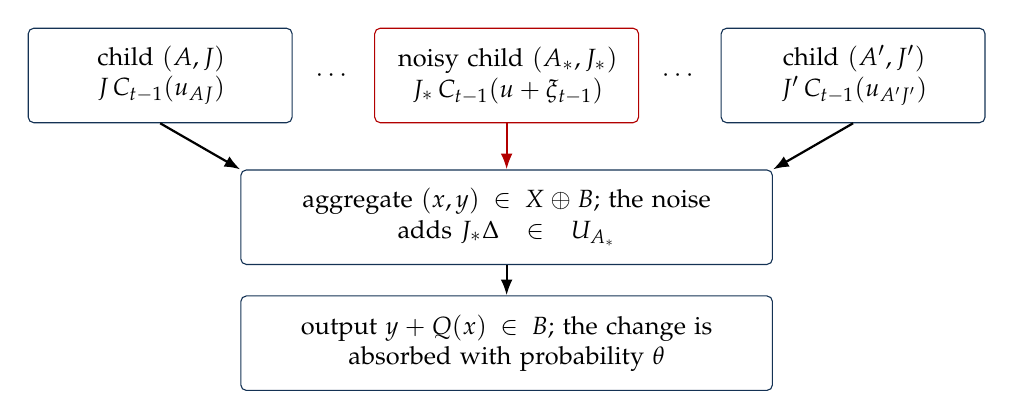
\begin{tikzpicture}[every node/.style={font=\small,align=center},
 block/.style={draw=linkblue!80!black,rounded corners=2pt,text width=3.0cm,inner sep=5pt,minimum height=12mm},
 flow/.style={-{Latex[length=2mm]},thick}]
\node[block] (l) at (0,0) {child $(A,J)$\\ $J\,C_{t-1}(u_{AJ})$};
\node[block,draw=red!70!black] (m) at (4.4,0) {noisy child $(A_*,J_*)$\\ $J_*\,C_{t-1}(u+\xi_{t-1})$};
\node[block] (r) at (8.8,0) {child $(A',J')$\\ $J'\,C_{t-1}(u_{A'J'})$};
\node at (2.2,0) {$\cdots$}; \node at (6.6,0) {$\cdots$};
\node[block,text width=6.4cm] (s) at (4.4,-1.8) {aggregate $(x,y)\in X\oplus B$; the noise\\ adds $J_*\Delta\in U_{A_*}$};
\node[block,text width=6.4cm] (o) at (4.4,-3.4) {output $y+Q(x)\in B$; the change is\\ absorbed with probability $\theta$};
\draw[flow] (l.south) -- (s.north west); \draw[flow,draw=red!70!black] (m)--(s);
\draw[flow] (r.south) -- (s.north east); \draw[flow] (s)--(o);
\end{tikzpicture}
\caption{One level of the tree. Every child output is embedded into an update
space $U_A$, the embedded outputs are summed, and one quadratic block is applied.
Only the randomly selected child carries noise.}
\label{fig:tree}
\end{figure}

\begin{lemma}[Nonlinear stability; Lemma~3.7 of \cite{OpenAI-UGC}]\label{lem:tree-noise}
For uniform $u\in P_t$,
$p_t:=\Pr[C_t(u+\xi_t)\ne C_t(u)]=(1-q^{-3})(1-\theta)^t$.
\end{lemma}

\begin{proof}
At height $0$ this is the probability that a uniform symbol is nonzero.
Condition on the selected child and its output change $\Delta$. By
\eqref{eq:tree-equiv} the change is invariant under shifting that child's
input, while its initial output is translated by every element of $B$, so the
child's initial output is uniform given $\Delta$; all other child outputs are
independent and uniform. Since the aggregate map is onto, the initial aggregate
$(x,y)$ is uniform and independent of the update $J\Delta$. Given $\Delta\ne0$
and $A$, the isomorphism $J$ is still uniform, so $J\Delta$ is uniform in
$U_A\setminus\{0\}$, and \cref{lem:block-noise} gives change probability
$1-\theta$. Hence $p_t=(1-\theta)p_{t-1}$.
\end{proof}

\subsection{Linear observers of the tree}\label{sec:lifts}

To track linear observers we need to say what an observer ``restricting to
$z$ on the output'' means on a tree whose output translations are realized by
many different shifts.

\begin{definition}
For $S\le B^*$, a \emph{lift} on $P_t$ is a linear map $z\mapsto\psi_z$ from
$S$ to $P_t^*$ with $\psi_z|_{R_t}=z\circ\lambda_t$. It is \emph{full} if
$S=B^*$.
\end{definition}

\begin{lemma}[Factorization; Lemma~3.8 of \cite{OpenAI-UGC}]\label{lem:factor}
Given a lift on $P_t$ ($t\ge1$), there is a single linear
$\gamma\colon S\to X^*$ such that for every child $(A,J)$ the restriction of
$\psi_z$ to that child's shifts factors through $\lambda_{t-1}$ via the
character
\[
\phi_{AJ}(z)=J^*\bigl((\gamma_z,z)|_{U_A}\bigr)\in B^*.
\]
\end{lemma}

\begin{proof}[Proof idea]
A shift supported on one child with $\lambda_{t-1}=0$ is a parent shift of
output $0$, so $\psi_z$ kills it; hence $\psi_z$ restricted to child shifts
is a character of the child outputs. Summing these characters over children and
subtracting $z$ applied to the $B$-part of the aggregate gives something that
vanishes whenever the $X$-part of the aggregate vanishes, so it factors through
the $X$-part: that is $\gamma_z$.
\end{proof}

So descending into child $(A,J)$, the observer becomes $J^*\kappa_{A,\gamma}$,
with the same $\gamma$ for all children. Since $J^*$ is an isomorphism, the
rank after descending is the rank of $\kappa_{A,\gamma}$, and
\cref{lem:kernel,eq:rank-loss} apply. Choose a linear section of $\phi_{AJ}$ by a
fixed rule to get a lift on the child with domain $\im\phi_{AJ}$; every
functional obtained this way is a restriction of a member of the original
family.

\begin{proposition}[Detection at fixed $B$; Prop.~3.9 of \cite{OpenAI-UGC}]\label{prop:detect}
Let $s=\lfloor H_{r_0}/(8\theta)\rfloor$. Every full lift on $P_s$ detects
$\xi_s$ with probability at least $1/4$: some $\psi_z(\xi_s)\ne0$.
\end{proposition}

\begin{proof}
Restrict the lift to the generic space $S_\star$ of rank $r_0$ and follow the
random leaf path, descending the lift as above. Let $r_j$ be the rank after $j$
steps and $\Delta_j=H_{r_j}-H_{r_{j+1}}\ge0$.

\emph{Freshness.} Let $\mathcal F_j$ be the path choices before step $j$. Given
$\mathcal F_j$ and the next line $A_j$, the subspace
$E_j=\im\kappa_{A_j,\gamma_j}\le U_{A_j}^*$ is fixed, and the next domain is
$S_{j+1}=J_j^*E_j$. Because $J_j$ is a uniform isomorphism, $S_{j+1}$ is a
\emph{uniformly random} subspace of $B^*$ of that rank, so it is non-generic
with probability at most $\eps_0$. The next lift may depend on $J_j$, but
genericity controls \emph{every} $g$ at once, so this does no harm.

\emph{Potential.} Given $\mathcal F_j$, the line $A_j$ is uniform. If $S_j$ is
generic, $\E[\Delta_j\mid\mathcal F_j]\le3\theta$ by \eqref{eq:rank-loss}; if
not, a loss has probability $\le2^{r_0}\theta$ and size $\le H_{r_0}$. Averaging
with freshness, $\E\Delta_j\le(3+H_{r_0}2^{r_0}\eps_0)\theta\le4\theta$. Summing,
$\E[H_{r_0}-H_{r_s}]\le4s\theta\le H_{r_0}/2$. Extinction requires a drop of
$H_{r_0}$, so by Markov $\Pr[r_s=0]\le1/2$.

\emph{At the leaf}, $P_0=R_0=B$ and the lift consists of the surviving
characters themselves; an independent uniform symbol of $B$ is detected by a
rank-$r_s>0$ space with probability $1-2^{-r_s}\ge1/2$. The product is $1/4$.
\end{proof}

\subsection{From the tree to the gadget}\label{sec:enlarge}

\paragraph{Quotient.} Put $V_0=P_s/\ker\lambda_s$. By \eqref{eq:tree-equiv},
$C_s$ descends to $\bar C\colon V_0\to B$, and $R_s/\ker\lambda_s\cong B$
becomes an honest subspace $B\subseteq V_0$ with $\bar C(x+b)=\bar C(x)+b$.
Let $\nu$ be the image of the noise. Stability is unchanged, and pulling back
any $G_0\le V_0^*$ with $G_0|_B=B^*$ along a section gives a full lift, so
$G_0$ detects $\nu$ with probability $\ge1/4$.

\paragraph{Enlargement.} Fix $\ell\ge b+2$, $K=\F_2^\ell$, and let $\mathcal L$
be the set of all injective linear maps $L\colon B\to K$. Take one copy of $V_0$
for each $L$, put $\widetilde C((x_L)_L)=\sum_LL\,\bar C(x_L)$, and quotient by
the shifts of total output $0$; the result is $\V$ with $K\subseteq\V$ and
$C\colon\V\to K$ equivariant. The noise $\mu$ picks a uniform $L$ and adds a
sample of $\nu$ in that copy. Since $L$ is injective, $C$ changes exactly when
that copy's output does.

\paragraph{Detection with a fixed threshold.} Let $G\le\V^*$ with
$S=G|_K$ of dimension $r\ge r_*:=b+2$. On copy $L$, the restriction of $G$ to
that copy's $B$ is $L^*S$. This fails to be all of $B^*$ only if
$Lb'\in S^\perp$ for some nonzero $b'\in B$; for fixed $b'$ and uniform $L$,
$Lb'$ is a uniform nonzero vector, so this has probability $\le2^{-r}$, and a
union bound gives $\Pr_L[L^*S\ne B^*]\le2^{b-r}\le1/4$. On the remaining copies
detection is at least $1/4$, for a total of at least $\tfrac34\cdot\tfrac14\ge\tfrac18$.

\begin{proof}[Proof of \cref{thm:gadget}]
Choose $r_0$ with $\exp(1-H_{r_0}/8)\le p_*$, then $\eps_0$, $d$, $\theta$, $s$
as above. Stability: $p_s\le(1-\theta)^s\le e^{-\theta s}\le e^{\theta-H_{r_0}/8}\le p_*$.
Detection holds with $r_*=b+2=3d+2$, which depends only on $p_*$, for every
$\ell\ge r_*$. All objects are finite and can be found by enumeration.
\end{proof}

\begin{remark}[Size]
The gadget is enormous. $\abs{\mathcal I}$ is about $q^2\abs{GL_{3d}(\F_2)}\approx2^{9d^2}$,
the tree has depth $s\approx q^2\ln r_0/8$, so $\dim P_s$ is about
$3d\cdot2^{9d^2s}$, doubly exponential in $q$, and $\abs{\V}$ is exponential in
that. This does not matter for the theorem, where $\V$ is a constant, but it
makes the eventual polynomial running time astronomically large
(\cref{rem:galactic}).
\end{remark}

\section{The Unique Games instance}\label{sec:instance}

Fix gadget data $(\V,K,C,\mu)$ from \cref{thm:gadget}, with $K=\F_2^\ell$, and a
linear complement $\V=K\oplus W$. Fix a tuple length $k$ and the preprocessed
parity instance $\cE$ with weights $\omega$.

\subsection{Questions and answer spaces}

An \emph{equation question} is a tuple $U=(e_1,\dots,e_k)$ drawn from
$\omega^{\otimes k}$, with replacement. Its answers are the $k$-tuples of
satisfying assignments. Write an assignment to block $i$ by its first two bits
$(x_i,y_i)$; the third is $b_{e_i}+x_i+y_i$. Add a homogeneous coordinate
$t_0$ and set
\[
L_U=\F_2^{m},\qquad m=1+2k,
\]
so that the \emph{valid} answers are exactly the vectors with $t_0=1$. Write
$e_0^\top$ for the functional reading $t_0$. Repeated equations in different
blocks get separate local coordinates.

A \emph{projected question} $O$ is obtained from $U$ by independently, in each
block, keeping the equation with probability $1-\beta$, or with probability
$\beta$ keeping only one of its three variables, chosen uniformly. The
projection $\bpi\colon L_U\to L_O$ keeps $t_0$, is the identity on kept
equations, and sends a projected block to its retained bit:
\[
x_i,\qquad y_i,\qquad\text{or}\qquad b_{e_i}t_0+x_i+y_i .
\]
Note the $t_0$ term in the third case: the third variable is an \emph{affine}
function of the first two, which is why homogeneous coordinates are used.

\subsection{Tables and exact keys}\label{sec:keys}

A \emph{table} on a question $Q$ (equation or projected) is a linear map
$P\in\Hom(L_Q,\V)$, equivalently an affine map from valid answers to $\V$.
Write it as $P=c\,t_0+\sum_i(a_ix_i+d_iy_i)$ on an equation question, with
intercept $c$ and block slopes $(a_i,d_i)\in\V^2$.

The soundness proof will compare a tuple $U$ with its projection $O$, and
needs the labeling's answer on a table $P'$ for $O$ to coincide with its
answer on the pulled-back table $P'\bpi$ for $U$. Rather than test this, the
construction makes the two tables literally the same vertex. The device is a
canonical form, the \emph{key}, which records only the coordinates a table
actually depends on.

\paragraph{Reducing a block.} In an equation block look at the rank of the
slope map $(x_i,y_i)\mapsto a_ix_i+d_iy_i$:
\begin{itemize}
\item rank $2$: keep the equation and its slopes;
\item rank $0$: drop the block;
\item rank $1$: the slopes are $(v,0)$, $(0,v)$ or $(v,v)$ for some $v\ne0$,
  so the table depends on the block only through one actual variable, at
  position $1$, $2$ or $3$. Record that variable and the slope $v$. In the third
  case $v(x_i+y_i)=v\,z_i+b_{e_i}v\,t_0$, where $z_i$ is the third bit, so add
  $b_{e_i}v$ to the intercept.
\end{itemize}
In a singleton block of a projected question, keep the variable if its slope is
nonzero and drop it otherwise.

\begin{definition}[Key]
The \emph{support} of $(Q,P)$ is the list of kept blocks, with their positions
in $[k]$, their tags (equation or variable) and their IDs. The \emph{key} is the
support together with the reduced affine table on it, including the corrected
intercept $\tilde c=c+\sum_{i\in J_3}b_{e_i}v_i$, where $J_3$ is the set of
blocks reduced to their third variable.
\end{definition}

\begin{lemma}[Pullbacks share keys; \S4.3 of \cite{OpenAI-UGC}]\label{lem:keys}
For every permitted projection $\bpi\colon L_U\to L_O$ and every table $P'$ on $O$,
the tables $(U,P'\bpi)$ and $(O,P')$ have the same key.
\end{lemma}

\begin{proof}
Kept equations contribute identically. A singleton of slope $0$ disappears on
both sides. A singleton of nonzero slope $v$ at position $j$ pulls back to the
rank-one pattern $(v,0)$, $(0,v)$ or $(v,v)$, which reduces to the same variable
at the same position. For position $3$, the pullback adds $b_ev$ to the
intercept (from the $b_et_0$ term of $\bpi$), and the reduction adds $b_ev$ again;
over $\F_2$ the two cancel.
\end{proof}

\begin{example}
Take $k=1$, one equation $x+y+z=1$, and a table on $U$ with slopes $(v,v)$ and
intercept $c$, so $P(x,y)=c+v(x+y)$. On valid answers $z=1+x+y$, so
$P=(c+v)+vz$: the key records ``variable $z$, slope $v$, intercept $c+v$''. The
projected question $O$ that keeps only $z$, with table $P'(z)=(c+v)+vz$, pulls
back to $(c+v)+v(1+x+y)=c+v(x+y)$, the same table, with the same key.
\end{example}

\subsection{Folding and vertices}

Translating a key by $h\in K$ means adding $h$ to its reduced intercept (realized
by replacing $P$ with $P+h\,e_0^\top$). This action is free, and the
\emph{vertices} of the instance are its orbits; each is represented by the key
whose intercept has zero $K$-component. For a table $P$ on $Q$ let $v(Q,P)$ be
the vertex and $c(Q,P)\in K$ the removed $K$-component. A labeling
$\lambda\colon\text{vertices}\to K$ defines the \emph{restored answer}
\[
F_Q(P)=\lambda(v(Q,P))+c(Q,P),
\]
and by construction and \cref{lem:keys}
\begin{equation}\label{eq:fold-share}
F_Q(P+h\,e_0^\top)=F_Q(P)+h\quad(h\in K),\qquad F_U(P'\bpi)=F_O(P').
\end{equation}
These two identities, \emph{folding} and \emph{sharing}, are the only
properties of the vertex construction the soundness proof uses.

\subsection{The test, and completeness}

The instance $\cG$ samples, independently,
\[
U\sim\omega^{\otimes k},\qquad P\in\Hom(L_U,\V)\text{ uniform},\qquad
a\sim\mu,\qquad l\in\F_2^m\text{ uniform},
\]
and checks
\begin{equation}\label{eq:test}
F_U(P)=F_U(P+a\,l^\top).
\end{equation}
In terms of the labeling this reads $\lambda(v_1)=\lambda(v_0)+c_0+c_1$, a
translation constraint on $K$. The weights are the sampling probabilities. The
projected questions $O$ do not appear in the test; they exist only in the
analysis.

\begin{lemma}[Completeness; Lemma~4.3 of \cite{OpenAI-UGC}]\label{lem:complete}
If $\OPT(\cE)\ge1-\xi$, then $\val(\cG)\ge1-k\xi-p_*/2$.
\end{lemma}

\begin{proof}
Fix a global assignment of value $\ge1-\xi$. It gives an answer on every
support: the global bit on a singleton; on an equation, its first two global
bits and the third bit that satisfies the equation. Label each orbit
representative by applying $C$ to its reduced table evaluated at this answer.
By equivariance of $C$, the restored answer of any table is then $C$ of the
table evaluated at the support answer.

With probability $\ge1-k\xi$ every equation in $U$ is satisfied, and then all
support answers are projections of one full answer $z_U\in L_U$ with $t_0=1$.
The two sides of \eqref{eq:test} become $C(Pz_U)$ and
$C(Pz_U+a(l^\top z_U))$. Since $z_U\ne0$, $Pz_U$ is uniform in $\V$ and
independent of $(a,l)$, and $l^\top z_U$ is a fair coin, so the test fails with
probability at most $p_*/2$.
\end{proof}

The honest labeling is a function of the key only, which is why it is
well-defined on vertices: two tables with the same key have the same support,
hence the same support answer.

\section{The plan for soundness}\label{sec:plan}

Soundness means: on a NO instance, no labeling passes \eqref{eq:test} with
probability $0.99$. As in the 2-to-2 proof, this is shown by playing two bounds
against each other in an auxiliary two-player game with \emph{advice}.

\subsection{Parameters}

The constants are chosen in this order, each depending only on the earlier ones:
\begin{enumerate}
\item $p_*>0$, and the gadget threshold $r_*$ (\cref{thm:gadget});
\item $\eta=2^{-r_*}/16$;
\item from the inverse shortcode theorem (\cref{thm:inverse}), $\alpha\in(0,1]$
  and $\rs\ge1$ depending on $\eta$;
\item $\ell$ large enough for the inverse theorem and the gadget, with
  $2^{-(\ell-\rs)}<\alpha/8$ and $2^{-\ell}<\eta/4$; then the gadget
  $(\V,K,C,\mu)$ and a splitting $\V=K\oplus W$;
\item the tuple length $k$, a perfect cube, and $\beta=k^{-2/3}$.
\end{enumerate}
Write a table as $P=(M,T)$ with $M\colon L_U\to K$ and $T\colon L_U\to W$. The
$K$-part $M$ is an $\ell\times m$ binary matrix, and the BKS shortcode lives
on it.

\subsection{The advice game}

\begin{definition}[Projected advice experiment; Def.~5.2 of \cite{OpenAI-UGC}]\label{def:advice}
Sample $U$, $O$ and $\bpi$ as in \cref{sec:instance}; a uniform linear map
$A\colon K\to\F_2^{\rs}$; and uniform tables $T_O\colon L_O\to W$ and
$M_O\colon L_O\to K$. Put $S_O=AM_O$. The two players receive
\[
\text{$U$-player: }(U,\ A,\ T_O\bpi,\ S_O\bpi),\qquad
\text{$O$-player: }(O,\ A,\ T_O,\ S_O),
\]
and each returns a valid answer for its own question. They win if
$\bpi(a_U)=a_O$.
\end{definition}

Both players see the $W$-part of the table and $\rs$ random linear combinations
of the rows of the $K$-part, pulled back appropriately; neither sees the rest of
$M_O$. The advice has bounded dimension per block, $\dim W+\rs$, independent of
$k$, and that is what the upper bound exploits.

\begin{idea}[Why advice?]
The inverse theorem will say that a good labeling, restricted to a typical
$(U,T)$, agrees with an affine function on a \emph{slice} of matrices cut out by
a few row conditions $d_i^\top M=s_i^\top$ and column conditions $Mq_j=t_j$. To
turn that into an answer, a player must know which slice it is in. Column
conditions are about answers (the $q_j$ live in $L_U$), but row conditions are
about the table. Giving both players the values of a few random row
combinations $AM$ lets them locate a row fiber, and \cref{sec:abundance} shows
that a random fiber is useful with constant probability. This is the
``advice'' idea of Khot--Minzer--Safra and Minzer--Zheng.
\end{idea}

\subsection{The two bounds}

\begin{proposition}[Decoding lower bound; Prop.~5.3 of \cite{OpenAI-UGC}]\label{prop:decode}
There are $\gamma>0$ and $k_0$, depending only on the fixed data of items
1--4, such that for every cube $k\ge k_0$ and every parity instance: if a family
of functions $F_Q\colon\Hom(L_Q,\V)\to K$ satisfies folding and sharing
\eqref{eq:fold-share} and passes \eqref{eq:test} with probability $\ge0.99$,
then the advice experiment with $\beta=k^{-2/3}$ has strategies that win with
probability $\ge\gamma$.
\end{proposition}

\begin{lemma}[Repetition upper bound; Lemma~6.2 of \cite{OpenAI-UGC}]\label{lem:clean}
If $\OPT(\cE)\le4/5$, every pair of strategies in the advice experiment wins
with probability at most
\[
\Bigl(1-\frac{\beta\,2^{-\dim W-\rs}}{3600}\Bigr)^k
\le\exp\Bigl(-\frac{2^{-\dim W-\rs}}{3600}\,k^{1/3}\Bigr).
\]
\end{lemma}

\begin{proposition}[A fixed gap; Prop.~6.3 of \cite{OpenAI-UGC}]\label{prop:gap}
For every sufficiently large cube $k$,
\[
\OPT(\cE)\ge1-\xi\ \Rightarrow\ \val(\cG)\ge1-k\xi-p_*/2,\qquad
\OPT(\cE)\le4/5\ \Rightarrow\ \val(\cG)\le99/100 .
\]
The threshold on $k$ depends only on the fixed data, not on $\cE$ or $\xi$.
\end{proposition}

\begin{proof}
Completeness is \cref{lem:complete}. Every labeling yields a family with
folding and sharing. If it passed with probability $\ge0.99$,
\cref{prop:decode} would give winning probability $\ge\gamma$, but for large
$k$ the bound of \cref{lem:clean} is below $\gamma$.
\end{proof}

With \cref{cor:amplify}, \cref{prop:gap} proves \cref{thm:ugc}; the bookkeeping
is in \cref{sec:finish}. Note that the NO bound $99/100$ does not depend on
$p_*$: the gadget's completeness can be made as good as desired without
touching soundness.

The proof of \cref{prop:decode} has three steps:
\begin{enumerate}
\item \textbf{Spectral comparison} (\cref{sec:spectral}): high acceptance of the
  latent test implies acceptance $\ge0.9\cdot2^{-r_*}$ of the ordinary BKS test
  on the $K$-part, for typical $(U,T)$.
\item \textbf{Structure and abundance} (\cref{sec:inverse}): by the inverse
  shortcode theorem and an erasure argument, a random row fiber is ``good''
  with constant probability, and each good fiber determines a short list of
  valid answers.
\item \textbf{Transfer and decoding} (\cref{sec:decoding}): the structure
  survives the passage from $U$ to its projection $O$, and a Fourier sampling
  rule for the $O$-player hits the projection of the $U$-player's list.
\end{enumerate}

\section{From the latent test to the ordinary shortcode test}\label{sec:spectral}

This is the step where the gadget is used, and it is short.

\begin{lemma}[Spectral comparison; Lemma~5.4 of \cite{OpenAI-UGC}]\label{lem:spectral}
If the family passes \eqref{eq:test} with probability $\ge0.99$, then
\[
\E_{U,T}\ \Pr_{M,a,l}\bigl[F_U(M,T)=F_U(M+al^\top,T)\bigr]\ \ge\ 0.9\cdot2^{-r_*},
\]
where now $a$ is uniform in $K$, and $M$, $T$, $l$ are uniform. Consequently at
least a $10\eta$ fraction of pairs $(U,T)$ have inner probability $\ge4\eta$.
\end{lemma}

\begin{proof}
Fix $U$. For a character $\sigma\in K^*$ let
$f_\sigma(P)=(-1)^{\sigma(F_U(P))}$; then
$\Pr[F_U(P)=F_U(P')]=\E_\sigma\,\E[f_\sigma(P)f_\sigma(P')]$ for uniform
$\sigma$. Fourier-expand $f_\sigma$ on $\Hom(L_U,\V)\cong\V^m$: the characters
are indexed by $g=(g_0,\dots,g_{m-1})\in(\V^*)^m$, with
$\chi_g(P)=(-1)^{\sum_ig_i(Pe_i)}$. Adding $al^\top$ multiplies $\chi_g$ by
$(-1)^{\sum_il_ig_i(a)}$. Averaging over uniform $l$ gives $1$ if all
$g_i(a)=0$ and $0$ otherwise, so for any noise law the acceptance is
\[
\E_{U,\sigma}\sum_g\abs{\widehat f_\sigma(g)}^2\,\Lambda_g,\qquad
\Lambda_g=\Pr_a[\,g_i(a)=0\ \forall i\,]\in[0,1].
\]
The multipliers are nonnegative, which is what makes the comparison work.

\emph{Latent noise.} For $a\sim\mu$, the gadget's detection property applied to
$G=\Span\{g_i\}$ gives $\Lambda_g\le7/8$ whenever
$\operatorname{rk}(g):=\dim\Span\{g_i|_K\}\ge r_*$. If $\mathsf{B}$ is the
average Fourier mass on such ``high-rank'' $g$, then $0.99\le1-\mathsf{B}/8$, so
$\mathsf{B}\le0.08$: at least $0.92$ of the mass is on $\operatorname{rk}(g)<r_*$.

\emph{Uniform noise in $K$.} For $a$ uniform in $K$,
$\Lambda_g=2^{-\operatorname{rk}(g)}\ge2^{-(r_*-1)}$ on low-rank $g$. Dropping
the (nonnegative) high-rank terms, acceptance is at least
$0.92\cdot2^{1-r_*}\ge0.9\cdot2^{-r_*}$. A perturbation in $K$ changes only the
$K$-part $M$ and leaves $T$ fixed, so this is the average over $(U,T)$ of the
ordinary BKS equality test applied to $M\mapsto F_U(M,T)$.

The average is $0.9\cdot2^{-r_*}=14.4\eta$. If a $q$ fraction of pairs have
inner probability $\ge4\eta$, then $14.4\eta\le4\eta+q$, so $q\ge10\eta$.
\end{proof}

\begin{idea}[What just happened.]
The gadget cannot make dishonest labelings fail outright; it only damps their
high-rank Fourier mass by a constant factor $7/8$. That is enough because the
target soundness is a fixed $0.99$, not a small $\delta$. Since $r_*$ was fixed
before $\ell$, the conclusion is an equality-test acceptance of order
$2^{-r_*}$, a constant that does not shrink as the alphabet grows, which is
exactly what the KMS inverse theorem needs.
\end{idea}

\section{Structure: the inverse theorem and good advice}\label{sec:inverse}

\subsection{The inverse shortcode theorem}

A \emph{slice} of $\Mat_{\ell,m}$ is a nonempty set
\[
\cS=\{M:\ d_i^\top M=s_i^\top\ (i\le n_r),\ \ Mq_j=t_j\ (j\le n_c)\},
\]
cut out by $n_r$ row conditions and $n_c$ column conditions.

\begin{theorem}[Inverse shortcode theorem; Thm.~5.1 of \cite{OpenAI-UGC}]\label{thm:inverse}
For every $\eta\in(0,1)$ there are $\alpha\in(0,1]$, $\rs\ge1$ and $\ell_0$ such
that for all $\ell\ge\ell_0$ and all $m\ge m_0(\eta,\ell)$: if
$f\colon\Mat_{\ell,m}\to\F_2^\ell$ satisfies
$\Pr_{M,a,l}[f(M)=f(M+al^\top)]\ge\eta$, then there are a slice $\cS$ with
$n_r,n_c\le\rs$ and $z\in\F_2^m$, $u\in\F_2^\ell$ with
$\Pr_{M\in\cS}[f(M)=Mz+u]\ge\alpha$.
\end{theorem}

\begin{proof}[Derivation from Grassmann expansion]
Equality acceptance is the mass-weighted average of how well each level set
$f^{-1}(y)$ is preserved by a random rank-one step, so some level set $S$ is
preserved with probability $\ge\eta$. Map each matrix to the
$\ell$-dimensional subspace $L_M=\{(x,M^\top x)\}\subseteq\F_2^{\ell+m}$. Then
$\dim(L_M\cap L_N)=\ell-\rank(M-N)$, so rank-one steps are exactly Grassmann
edges inside this chart, and exactly half of each vertex's Grassmann neighbors
lie in the chart. Hence $\{L_M:M\in S\}$ has Grassmann edge retention at least
about $\eta/4$. The Khot--Minzer--Safra theorem~\cite{KMS23} says such a set has
density $\ge\alpha(\eta)$ inside some ``zoom-in/zoom-out'' interval
$\{L:A_0\subseteq L\subseteq B_0\}$ with $\dim A_0+\operatorname{codim}B_0\le\rs$.
In matrix coordinates, $A_0\subseteq L_M$ is a set of row conditions and
$L_M\subseteq B_0$ a set of column conditions. On that slice $f$ equals the
constant $y$ on an $\alpha$ fraction, which is the claim with $z=0$.
\end{proof}

The proof gives $z=0$. Nonzero targets $z$ appear only after the column
conditions are used to shift $z$ (\cref{lem:answer-set}).

\subsection{Abundance of good advice}\label{sec:abundance}

The inverse theorem gives one good slice for each good $(U,T)$. But the
$U$-player sees only a \emph{random} row fiber $\{M:AM=AM_{\text{actual}}\}$,
and a specific fiber is hit with probability about $2^{-\rs m}$, which vanishes as
$k$ grows. The next lemma shows that good fibers are, in aggregate, abundant.

\begin{definition}
Row advice $(U,T,A,S_0)$ is \emph{good} if there are at most $\rs$ column
conditions and a target $Mz+u$ such that the set of $M$ satisfying both
$AM=S_0$ and the column conditions is nonempty and
$F_U(M,T)=Mz+u$ on at least an $\alpha/2$ fraction of it.
\end{definition}

\begin{lemma}[Good advice is common; Lemma~5.5 of \cite{OpenAI-UGC}]\label{lem:abundant}
For large $k$, if the family passes \eqref{eq:test} with probability $\ge0.99$,
then
\[
\Pr_{U,T,A,M}\bigl[(U,T,A,AM)\text{ is good}\bigr]\ \ge\ g_0:=10\,\eta^2\,2^{-\ell\rs}.
\]
\end{lemma}

\begin{proof}
Fix $(U,T)$ with inner acceptance $\ge4\eta$ (\cref{lem:spectral}) and write
$f(M)=F_U(M,T)$. Let $\mathsf{B}$ be the union of all good row fibers, over all
$A$ and $S_0$. Suppose $\Pr[\mathsf{B}]<\eta$.

\emph{Erase.} Replace $f$ on $\mathsf{B}$ by independent uniform values. Both
endpoints of a test step are uniform matrices, so acceptance drops by at most
$2\Pr[\mathsf{B}]$, leaving at least $2\eta$.

\emph{The erased values match nothing.} A slice with at most $\rs$ row and
$\rs$ column conditions has at least $2^{(\ell-\rs)(m-\rs)}$ elements, and there
are at most $2^{(2\rs+1)(\ell+m)}$ slice-and-target descriptions. For each, the
expected number of random matches is at most $2^{-\ell}\abs{\cS}<\alpha\abs\cS/8$, and
Hoeffding plus a union bound show that, for large $m$, some choice of erased
values contributes fewer than $\alpha\abs\cS/4$ matches to \emph{every} slice and
target.

\emph{Contradiction.} Take any slice of the allowed type and any target. Its
row conditions define a row fiber for some $A$ (pad with zero rows). If that
fiber was good, all of it was erased, and agreement is $<\alpha/4$. If it was
not good, the original agreement was $<\alpha/2$, and erasure adds $<\alpha/4$.
Either way agreement is $<\alpha$, contradicting \cref{thm:inverse} for the
modified function, whose acceptance is $\ge2\eta$. (The inverse theorem does
not need folding, so erasure is harmless.)

So $\Pr[\mathsf{B}]\ge\eta$. Each $M\in\mathsf{B}$ lies in a good fiber for some
particular $A$, which a uniform $A$ hits with probability $2^{-\ell\rs}$. Averaging
over the $\ge10\eta$ good pairs $(U,T)$ gives the bound.
\end{proof}

\subsection{Folding turns a slice into answers}

\begin{lemma}[The answer set; Lemma~5.5 of \cite{OpenAI-UGC}, second part]\label{lem:answer-set}
For good advice, fix (by a deterministic rule depending only on the advice and
the family) a witness: column conditions $Mq_j=t_j$ and a target $Mz+u$. Let
$Z=\Span\{q_j\}$. Then $z$ can be chosen with $e_0^\top z=1$, and
\[
\cA=(z+Z)\cap\{v:\ e_0^\top v=1\}
\]
is a nonempty set of valid answers of size at most $2^{\rs}$.
\end{lemma}

\begin{proof}
On the slice $Mw$ is fixed for $w\in Z$, so replacing $z$ by $z+w$ and $u$ by
$u+Mw$ does not change the target. Suppose every vector of $z+Z$ had $t_0=0$.
For $h\in H=\ker A$, the shift $M\mapsto M+h\,e_0^\top$ preserves the row fiber
(as $Ah=0$), the column conditions (as $e_0^\top q_j=0$) and the target (as
$e_0^\top z=0$), while folding shifts $F_U$ by $h$. Each orbit of this free
action contains at most one agreeing matrix, so agreement is at most
$\abs{H}^{-1}\le2^{-(\ell-\rs)}<\alpha/8$, contradicting goodness.
\end{proof}

\begin{idea}[Folding is what makes answers appear.]
The inverse theorem by itself only says ``$f$ is constant on a slice''.
Folding forbids $f$ from being constant along the direction $e_0^\top$, so the
slice must pin down the table along some answer-like vector with $t_0=1$.
Those vectors are the decoded answers. This is the matrix version of the
standard fact that a folded long code cannot be biased toward the empty set.
\end{idea}

\section{Transfer and Fourier decoding}\label{sec:decoding}

So far the $U$-side tables were uniform. In the advice experiment the
$U$-player's table is a padded table $(M_O\bpi,T_O\bpi)$ from $O$. The
choice $\beta=k^{-2/3}$ makes these almost the same.

\subsection{Padded tables look uniform}

\begin{lemma}[Lemma~5.6 of \cite{OpenAI-UGC}]\label{lem:tv}
For every $U$, averaging over the projection choices, the law of
$(M_O\bpi,T_O\bpi)$ is within total variation $o(1)$ of the uniform law on
$\Hom(L_U,\V)$ as $k\to\infty$ along cubes, uniformly in $U$ and the instance.
\end{lemma}

\begin{proof}
Let $n=\abs\V$. In a kept block the two slopes are independent uniform elements
of $\V$ (law $P_0$). In a projected block the pulled-back slopes are
$(a,0)$, $(0,a)$ or $(a,a)$ with $a$ uniform, each with probability $1/3$
(law $Q_0$). The likelihood ratio $dQ_0/dP_0$ is $n$ at $(0,0)$, $n/3$
at the other $3(n-1)$ points of the three lines, and $0$ elsewhere, so
$\chi^2(Q_0\|P_0)=(n-1)/3$. The block mixture $(1-\beta)P_0+\beta Q_0$ has
$\chi^2=\beta^2(n-1)/3$ from $P_0$, and over $k$ independent blocks
\[
\chi^2=\Bigl(1+\tfrac{n-1}{3}\beta^2\Bigr)^k-1\to0,\qquad\text{since }k\beta^2=k^{-1/3}\to0 .
\]
Total variation is at most $\frac12\sqrt{\chi^2}$. The intercept stays uniform
because the extra terms $b_ea$ from third-position projections are added to an
independent uniform intercept.
\end{proof}

\begin{idea}[The two jobs of $\beta=k^{-2/3}$.]
$k\beta^2\to0$ makes padded tables indistinguishable from uniform ones, so
everything proved for uniform tables transfers. $k\beta\to\infty$ makes the
number of projected blocks grow, which the repetition bound in
\cref{sec:clean} needs. Any $\beta$ with $k^{-1}\ll\beta\ll k^{-1/2}$ would
do.
\end{idea}

\subsection{The witness survives projection}

A column condition $Mq=t$ on $U$ becomes $M_O(\bpi q)=t$ on $O$. This can be
inconsistent (if $\bpi q=0\ne t$), so survival must be argued.

\begin{lemma}[Transfer; Lemma~5.7 of \cite{OpenAI-UGC}]\label{lem:transfer}
For large cubes $k$, with probability at least
$\gamma_1=\frac{\alpha g_0}{8}2^{-\ell\rs}$ over the joint data
$D=(U,O,\bpi,A,T_O,S_O)$, the $U$-player's advice is good, and its witness
transfers to a nonempty slice $\{M_O:\ AM_O=S_O,\ M_O\bpi q_j=t_j\}$ on which
$F_O(M_O,T_O)=M_O\bpi z+u$ with probability at least $\alpha/4$.
\end{lemma}

\begin{proof}
Under uniform sampling on $U$, let $\mathcal J$ be ``the advice is good and $M$
satisfies its column conditions'' and $\mathcal M$ ``$F_U(M,T)$ hits the
target''. A good fiber's column slice costs at most $\ell\rs$ extra linear
conditions, so $\Pr[\mathcal J]\ge g_02^{-\ell\rs}$ and
$\Pr[\mathcal J\cap\mathcal M]\ge\frac\alpha2\Pr[\mathcal J]$, giving
\[
\Pr[\mathcal J\cap\mathcal M]-\tfrac\alpha4\Pr[\mathcal J]\ \ge\ \tfrac{\alpha g_0}{4}2^{-\ell\rs}.
\]
Both events depend only on $(U,A,M,T)$, so by \cref{lem:tv} the same holds, up
to $o(1)$, with the padded table; for large $k$ the difference is at least
$\gamma_1$. Now condition on $D$: the remaining $M_O$ is uniform on its row
fiber, and sharing gives $F_U(M_O\bpi,T_O\bpi)=F_O(M_O,T_O)$. The padded
difference becomes $\E_D[p_D(q_D-\alpha/4)]$, where $p_D$ is the probability of
the transferred slice and $q_D$ the agreement on it. Since the integrand is at
most $1$ and is nonpositive unless $p_D>0$ and $q_D\ge\alpha/4$, that event has
probability $\ge\gamma_1$.
\end{proof}

\subsection{The two decoders}

\paragraph{The $U$-player.} From its advice it computes (by the fixed rule) the
witness and answer set $\cA$ of \cref{lem:answer-set}, and outputs a uniform
element of $\cA$; if the advice is not good it outputs any valid answer.

\paragraph{The $O$-player.} It never sees the $U$-player's witness. Let
$H=\ker A\le K$. Choose a representative $M_0$ with $AM_0=S_O$, so the row
fiber is $M_0+X$ with $X=\Hom(L_O,H)$. Pick a uniform $\sigma\in K^*$, form
$f_\sigma(N)=(-1)^{\sigma(F_O(M_0+N,T_O))}$ on $X$, and sample a frequency
$\Phi\in X^*=H^*\otimes L_O$ with probability $\abs{\widehat f_\sigma(\Phi)}^2$.
If $\sigma|_H\ne0$, pick $h\in H$ with $\sigma(h)=1$ and output the contraction
$\Phi(h)\in L_O$.

The output is always valid: folding gives
$f_\sigma(N+h\,e_0^\top)=-f_\sigma(N)$ when $\sigma(h)=1$, so every $\Phi$ with
nonzero coefficient has $\ip{\Phi}{h\,e_0^\top}=1$, that is,
$e_0^\top\Phi(h)=1$. This is Fourier list decoding in the style of
H{\aa}stad and Khot--Safra, run on the row fiber the advice reveals.

\begin{lemma}[Agreement; Lemma~5.8 of \cite{OpenAI-UGC}]\label{lem:agree}
On the data of \cref{lem:transfer}, the two decoders agree with probability
at least $2^{-\ell\rs}(\alpha/8)^2\,2^{-\rs}$.
\end{lemma}

\begin{proof}
Let $z'=\bpi z$ and $Z'=\bpi Z$, so $\bpi\cA=(z'+Z')\cap\{t_0=1\}$. On the
transferred slice $N|_{Z'}$ is a fixed map $b$. Define
$C_\sigma=\E[f_\sigma(N)(-1)^{\sigma(Nz')}\mid N|_{Z'}=b]$. Expanding the
agreement $\ge\alpha/4$ in characters of $K$ gives
$\E_\sigma\abs{C_\sigma}\ge\alpha/4$; discarding the $\le2^{-(\ell-\rs)}<\alpha/8$
fraction of $\sigma$ trivial on $H$ leaves
$\E_\sigma[\mathbf 1_{\sigma|_H\ne0}\abs{C_\sigma}]\ge\alpha/8$.

Since $(-1)^{\sigma(Nz')}$ is the character $\theta_\sigma=\sigma|_H\otimes z'$
and the slice is a coset of $\{N:N|_{Z'}=0\}$, whose annihilator is
$H^*\otimes Z'$, $C_\sigma$ is a signed sum of $\widehat f_\sigma(\Phi)$ over
$\Phi\in\theta_\sigma+H^*\otimes Z'$, a coset of size at most $2^{\ell\rs}$.
Cauchy--Schwarz twice gives
\[
\E_\sigma\Bigl[\mathbf 1_{\sigma|_H\ne0}\!\!\sum_{\Phi\in\theta_\sigma+H^*\otimes Z'}\!\!\abs{\widehat f_\sigma(\Phi)}^2\Bigr]
\ \ge\ 2^{-\ell\rs}(\alpha/8)^2 .
\]
Any such $\Phi=\sigma|_H\otimes z'+\Psi$ with $\Psi\in H^*\otimes Z'$ has
$\Phi(h)=z'+\Psi(h)\in z'+Z'$, and it is valid, so $\Phi(h)\in\bpi\cA$. The
$U$-player independently picks a preimage with probability $\ge1/\abs\cA\ge2^{-\rs}$.
\end{proof}

\begin{proof}[Proof of \cref{prop:decode}]
Combine \cref{lem:transfer,lem:agree}:
$\gamma=\gamma_1\,2^{-\ell\rs}(\alpha/8)^2\,2^{-\rs}$, independent of $k$ and of
the instance. The strategies need not be efficient; they only bound the
value of a finite game.
\end{proof}

\section{Clean coordinates and the repetition bound}\label{sec:clean}

It remains to prove \cref{lem:clean}: on a NO instance every pair of
strategies in the advice game wins with probability $\exp(-\Omega(k^{1/3}))$.
The idea, from Khot--Minzer--Safra, is that on blocks where the advice happens to
carry no information, the players are just playing $G_\cE$ in parallel.

\begin{proof}[Proof of \cref{lem:clean}]
Fix strategies. Condition on $A$, and combine the advice into
$D_O=(T_O,S_O)\colon L_O\to E_A:=W\oplus\im A$. Given the questions, the
intercept and every block slope of $D_O$ are independent and uniform in $E_A$,
whatever the equation IDs and positions are.

\emph{Clean blocks.} Call block $i$ \emph{clean} if it was projected to a
variable and its advice slope is $0$. Given $A$, blocks are clean independently
with probability $p_A=\beta/\abs{E_A}=\beta2^{-\dim W-\rank A}$, and
\[
\Pr[e_i=e,\ i\text{ clean at position }j\mid A]=\omega_e\cdot\tfrac13\cdot p_A,
\]
so a clean block's (equation, variable) pair has exactly the distribution of
$G_\cE$.

\emph{Freeze everything else.} Let $R$ consist of $A$, the clean set $I$, the
intercept of $D_O$, and, for each $i\notin I$, its equation, whether it was
projected, its position, and its slopes. Given $R=r$, the clean pairs
$(e_i,v_{e_i,j_i})_{i\in I}$ are independent samples of $G_\cE$.

\emph{Each player can rebuild its own input.} The $U$-player, given the clean
equations $(e_i)_{i\in I}$ and $r$, knows all of $U$. Its pulled-back slopes in
clean blocks are $(0,0)$; all other slopes and the full intercept
$c_U=c_O+\sum_{j_i=3}b_{e_i}d_i$ are determined by $r$, because clean blocks
contribute $d_i=0$. So it can reconstruct its entire advice. Symmetrically the
$O$-player, given the clean variables and $r$, reconstructs $O$ and its advice.
Neither needs the other's clean questions.

\emph{Reduce to repetition.} So for each $r$ we get strategies for
$G_\cE^{\otimes\abs I}$: rebuild the original input, run the original strategy,
and report the answers in the clean blocks. Winning the advice game implies
winning every clean block, so by \cref{thm:repetition} and \eqref{eq:base-gap}
(with $g=1/15$, $g^2/16=1/3600$)
\[
\Pr[\text{win}\mid R=r]\le\val\bigl(G_\cE^{\otimes\abs I}\bigr)\le(1-1/3600)^{\abs I}.
\]
Given $A$, $\abs I\sim\mathrm{Bin}(k,p_A)$, so averaging gives
$\E_A(1-p_A/3600)^k\le(1-\beta2^{-\dim W-\rs}/3600)^k$, using $\rank A\le\rs$,
and $k\beta=k^{1/3}$.
\end{proof}

\begin{idea}[Why the advice does not help a cheater.]
The advice has $\dim W+\rs$ bits per block, a constant. So a constant fraction
of projected blocks get zero advice, and with $k\beta=k^{1/3}$ projected blocks
there are $\Theta(k^{1/3})$ clean ones. On those, the advice is literally zero
on both sides, so it cannot correlate the players beyond what the base game
allows. Everything else is frozen and becomes shared randomness, which never
helps in a two-player game.
\end{idea}

\section{Putting it together}\label{sec:finish}

\subsection{The order of the parameters}

The proof is a long chain of ``for every \dots\ there is \dots'', and nearly
every subtlety is about ordering. \Cref{tab:params} lists the choices in the
order they are made. Each depends only on what is above it; in particular
nothing depends on the input formula.

\begin{table}[h]
\centering\small
\renewcommand{\arraystretch}{1.25}
\begin{tabular}{@{}r>{\raggedright}p{3.4cm}>{\raggedright\arraybackslash}p{8.2cm}@{}}
\toprule
& \textbf{Parameter} & \textbf{Chosen so that} \\
\midrule
1 & $\eps,\delta$ & given \\
2 & repetitions $t$ & $(1-1/10{,}240{,}000)^t\le\delta$ (depends on $\delta$ only)\\
3 & $p_*$, $\tau$ & $p_*\le\eps/t$, $\tau\le\min\{1/200,\eps/t\}$\\
4 & $r_0,\eps_0,d,s$; $r_*=3d+2$ & gadget stability $\le p_*$ (\cref{thm:gadget})\\
5 & $\eta=2^{-r_*}/16$; $\alpha,\rs$ & inverse shortcode theorem at $\eta$\\
6 & $\ell$; then $(\V,K,C,\mu)$, $W$ & $\ell\ge\ell_0$, $2^{-(\ell-\rs)}<\alpha/8$, $2^{-\ell}<\eta/4$\\
7 & $g_0,\gamma_1,\gamma$ & explicit in $\eta,\alpha,\rs,\ell$\\
8 & cube $k$, $\beta=k^{-2/3}$ & $m=1+2k\ge m_0$; erasure union bound $<1$; TV small; $e^{-ck^{1/3}}<\gamma$\\
9 & $\xi$ & $\xi<\min\{1/100,\ \eps/(2kt)\}$\\
10 & input $\varphi$ & H{\aa}stad($\xi$) $\to$ distinct positions $\to$ $\cG$ $\to$ subdivide($\tau$) $\to$ $t$-fold product\\
\bottomrule
\end{tabular}
\caption{Parameter order. The NO-case bound $0.99$ uses only rows 4--8 and holds for every $p_*$.}
\label{tab:params}
\end{table}

\begin{proof}[Proof of \cref{thm:ugc}]
With the choices of \cref{tab:params}, \cref{prop:gap} gives a weighted
translation game $H=\cG$ with YES value $\ge1-d$, $d=k\xi+p_*/2\le\eps/t$, and
NO value $\le99/100$. \Cref{cor:amplify} (rounding, subdivision and $t$-fold
repetition) gives the final instance: YES value
$\ge1-t(d+\tau)/4\ge1-\eps/2$ and NO value $\le\delta$, on the alphabet
$\F_2^{\ell t}$, simple, bipartite, with translation constraints.

\emph{Running time.} The game $\cG$ has one group of constraints for each of the
$N^k$ equation tuples, where $N$ is the number of equations, and a constant
number (depending on $\abs\V$ and $m$) of tables, noise values and vectors $l$
per tuple. Keys are computed by linear algebra in fixed dimension. Rounding
gives $O(h)$ edges and the $t$-fold product raises the size to a fixed power.
All of this is polynomial for fixed $\eps,\delta$.
\end{proof}

\begin{remark}[A galactic polynomial]\label{rem:galactic}
The exponent of the polynomial is at least $k$, and \cref{lem:tv} needs
$k\beta^2\abs\V=k^{-1/3}\abs\V\to0$, so $k\gg\abs\V^3$, where $\abs\V$ is
already a tower of exponentials in the gadget parameters. The reduction is
polynomial time in the complexity-theoretic sense only. For the consequences
below this is irrelevant: they are statements about NP-hardness.
\end{remark}

\section{Consequences}\label{sec:consequences}

\Cref{thm:ugc} turns the many results conditional on the UGC into NP-hardness
results. Section~8 of the manuscript states the precise forms and checks the
details needed to plug the theorem into each reduction. Among them:
\begin{itemize}
\item \textbf{Max-Cut:} approximating beyond the Goemans--Williamson ratio
  $\alpha_{\mathrm{GW}}\approx0.87856$ is NP-hard~\cite{KKMO07,GW95}.
\item \textbf{Vertex Cover:} approximating within any factor below $2$ is
  NP-hard~\cite{KhotRegev}.
\item \textbf{Every Max-CSP:} beating the basic SDP integrality ratio is
  NP-hard~\cite{Raghavendra08}.
\item \textbf{Ordering CSPs:} beating a random ordering is NP-hard for every
  fixed ordering predicate, following Guruswami, H{\aa}stad, Manokaran,
  Raghavendra and Charikar.
\item \textbf{Cuts and clustering:} Multicut, nonuniform Sparsest Cut,
  Min-2CNF$^{\equiv}$ Deletion and Correlation Clustering are NP-hard to
  approximate within every constant factor, following Chawla, Krauthgamer,
  Kumar, Rabani and Sivakumar.
\end{itemize}
The repository also contains direct proofs, not going through the UGC, of the
Max-Cut, Vertex Cover, Min-UnCut and directed feedback vertex set results.

\section{A guide for the careful reader}\label{sec:reader}

\subsection{What this note does and does not establish}

This note follows the manuscript's proof and does not add new mathematics. In
writing it I reworked the calculations reproduced above: the block lemmas and
the alignment criterion, the probability that a block absorbs an update, the
rank-loss and harmonic-potential bookkeeping, the enlargement step, the noise
eigenvalue computation and spectral comparison, the folding argument for the
answer set, the $\chi^2$ estimate, the clean-coordinate reconstruction
(including the intercept correction), and the final parameter arithmetic. I
found no errors in these. I did not referee every step at the level of detail
in the manuscript: the erasure argument's concentration bound, the
witness-transfer conditioning and the Fourier coset computation are presented
here in condensed form, and the external theorems (H{\aa}stad, KMS, Dinur--Steurer)
are taken as given. I did not run the Lean check (\cref{sec:lean}). If it
passes, it is far stronger evidence than any reading.

\subsection{Where to look hardest}

\begin{enumerate}
\item \textbf{The gadget} (\cref{sec:gadget}). This is the new idea and the
  one place where a conceptual error would sink everything. It is elementary
  and self-contained. Points worth checking: that the factorization of
  \cref{lem:factor} uses a single $\gamma$ for all children; that genericity
  must hold for \emph{every} $g$ because the descended lift may depend on the
  random isomorphism $J$; and that the threshold $r_*=b+2$ really is
  independent of $\ell$.
\item \textbf{Using the inverse theorem uniformly.} \Cref{thm:inverse} is
  applied to functions on very rectangular matrices ($\ell$ fixed,
  $m=1+2k\to\infty$) and to functions that are not folded (after erasure). The
  quantifiers $\ell\ge\ell_0(\eta)$, $m\ge m_0(\eta,\ell)$ allow both.
\item \textbf{Abundance} (\cref{lem:abundant}). The step from ``one good
  slice exists'' to ``random advice is good with constant probability'' is new
  relative to the 2-to-2 proof, and the reasoning summary shows the model
  identified it as a gap and repaired it.
\item \textbf{Exact keys} (\cref{lem:keys}). The intercept correction for
  third-position variables has to cancel exactly, and repeated equations across
  blocks must keep separate coordinates.
\item \textbf{Conditioning in \cref{lem:clean}.} The frozen data $R$ must not
  include anything correlated with the clean questions beyond the clean mask,
  and each player must be able to rebuild its input from its own clean
  questions alone.
\item \textbf{Parameter order} (\cref{tab:params}). In particular, $t$ is chosen
  before the alphabet, which requires alphabet-independent repetition.
\end{enumerate}

\subsection{Correspondence with the manuscript}

\begin{center}\small
\renewcommand{\arraystretch}{1.15}
\begin{tabular}{@{}ll@{}}
\toprule
\textbf{This note} & \textbf{Manuscript} \\
\midrule
\cref{thm:ugc} & Theorem 1.1 \\
\cref{lem:subdivide}, \cref{cor:amplify} & Lemma 7.1, \S7.2 \\
\cref{thm:parity}, \cref{lem:distinct}, \eqref{eq:base-gap} & Theorem 4.1, Lemma 4.2, Eq.~(4.1) \\
\cref{thm:gadget} & Lemma 3.1 \\
\cref{lem:block-basic,lem:block-noise,lem:kernel} & Lemmas 3.2--3.4 \\
\cref{lem:generic} & Definition 3.5, Lemma 3.6 \\
\cref{lem:tree-noise,lem:factor,prop:detect} & Lemmas 3.7--3.8, Proposition 3.9 \\
\cref{sec:enlarge} & \S3.5 \\
\cref{lem:keys}, \eqref{eq:fold-share} & \S4.3 \\
\cref{lem:complete} & Lemma 4.3 \\
\cref{def:advice}, \cref{prop:decode} & Definition 5.2, Proposition 5.3 \\
\cref{thm:inverse} & Theorem 5.1 \\
\cref{lem:spectral} & Lemma 5.4 \\
\cref{lem:abundant,lem:answer-set} & Lemma 5.5 \\
\cref{lem:tv,lem:transfer,lem:agree} & Lemmas 5.6--5.8 \\
\cref{thm:repetition}, \cref{lem:clean}, \cref{prop:gap} & Theorem 6.1, Lemma 6.2, Proposition 6.3 \\
\cref{sec:consequences} & Section 8 and Appendix A \\
\bottomrule
\end{tabular}
\end{center}

\subsection{Notation}

\begin{center}\small
\renewcommand{\arraystretch}{1.15}
\begin{tabular}{@{}ll@{}}
\toprule
$K=\F_2^\ell$ & the Unique Games alphabet before repetition \\
$\V\supseteq K$, $C$, $\mu$ & latent space, nonlinear decoder, latent noise \\
$p_*$, $r_*$ & gadget stability error and rank threshold \\
$U$, $O$, $\bpi$ & equation tuple, sparse projection, answer projection \\
$L_U=\F_2^{1+2k}$, $e_0^\top$ & homogeneous answer space, the $t_0$ coordinate \\
$P=(M,T)$ & table, split into $K$-part (a matrix) and $W$-part \\
$F_Q$ & restored answer of a labeling on question $Q$ \\
$\eta$, $\alpha$, $\rs$ & inverse-theorem input, agreement and slice size \\
$A$, $S_O=AM_O$ & advice map and advice rows \\
$\beta=k^{-2/3}$ & projection rate \\
\bottomrule
\end{tabular}
\end{center}


\bibliographystyle{plain}
\begin{thebibliography}{99}\small
\bibitem{OpenAI-UGC} OpenAI. \emph{The Unique Games Theorem.} Manuscript, September 23, 2026. \url{https://github.com/openai/math}.
\bibitem{BGS98} M.~Bellare, O.~Goldreich, M.~Sudan. Free bits, PCPs, and nonapproximability---towards tight results. \emph{SIAM J.\ Comput.} 27(3), 1998.
\bibitem{BKS18} B.~Barak, P.~Kothari, D.~Steurer. Small-set expansion in shortcode graph and the 2-to-2 conjecture. ITCS 2019; arXiv:1804.08662.
\bibitem{DKKMS} I.~Dinur, S.~Khot, G.~Kindler, D.~Minzer, M.~Safra. Towards a proof of the 2-to-1 games conjecture? STOC 2018.
\bibitem{DS14} I.~Dinur, D.~Steurer. Analytical approach to parallel repetition. STOC 2014.
\bibitem{GW95} M.~Goemans, D.~Williamson. Improved approximation algorithms for maximum cut and satisfiability problems using semidefinite programming. \emph{J.\ ACM} 42(6), 1995.
\bibitem{Hastad01} J.~H{\aa}stad. Some optimal inapproximability results. \emph{J.\ ACM} 48(4), 2001.
\bibitem{Khot02} S.~Khot. On the power of unique 2-prover 1-round games. STOC 2002.
\bibitem{KKMO07} S.~Khot, G.~Kindler, E.~Mossel, R.~O'Donnell. Optimal inapproximability results for MAX-CUT and other 2-variable CSPs? \emph{SIAM J.\ Comput.} 37(1), 2007.
\bibitem{KMS17} S.~Khot, D.~Minzer, M.~Safra. On independent sets, 2-to-2 games, and Grassmann graphs. STOC 2017.
\bibitem{KMS23} S.~Khot, D.~Minzer, M.~Safra. Pseudorandom sets in Grassmann graph have near-perfect expansion. FOCS 2018; \emph{Annals of Math.} 198(1), 2023.
\bibitem{KhotRegev} S.~Khot, O.~Regev. Vertex cover might be hard to approximate to within $2-\eps$. \emph{J.\ Comput.\ Syst.\ Sci.} 74(3), 2008.
\bibitem{KS13} S.~Khot, M.~Safra. A two-prover one-round game with strong soundness. \emph{Theory of Computing} 9, 2013.
\bibitem{MZ} D.~Minzer, K.~Zheng. Near optimal alphabet-soundness tradeoff PCPs. STOC 2024.
\bibitem{Rao11} A.~Rao. Parallel repetition in projection games and a concentration bound. \emph{SIAM J.\ Comput.} 40(6), 2011.
\bibitem{Raghavendra08} P.~Raghavendra. Optimal algorithms and inapproximability results for every CSP? STOC 2008.
\end{thebibliography}
\end{document}
